% Options for packages loaded elsewhere
\PassOptionsToPackage{unicode}{hyperref}
\PassOptionsToPackage{hyphens}{url}
\PassOptionsToPackage{dvipsnames,svgnames,x11names}{xcolor}
%
\documentclass[
  number,
  preprint,
  3p,
  onecolumn]{elsarticle}

\usepackage{amsmath,amssymb}
\usepackage{iftex}
\ifPDFTeX
  \usepackage[T1]{fontenc}
  \usepackage[utf8]{inputenc}
  \usepackage{textcomp} % provide euro and other symbols
\else % if luatex or xetex
  \usepackage{unicode-math}
  \defaultfontfeatures{Scale=MatchLowercase}
  \defaultfontfeatures[\rmfamily]{Ligatures=TeX,Scale=1}
\fi
\usepackage{lmodern}
\ifPDFTeX\else  
    % xetex/luatex font selection
\fi
% Use upquote if available, for straight quotes in verbatim environments
\IfFileExists{upquote.sty}{\usepackage{upquote}}{}
\IfFileExists{microtype.sty}{% use microtype if available
  \usepackage[]{microtype}
  \UseMicrotypeSet[protrusion]{basicmath} % disable protrusion for tt fonts
}{}
\makeatletter
\@ifundefined{KOMAClassName}{% if non-KOMA class
  \IfFileExists{parskip.sty}{%
    \usepackage{parskip}
  }{% else
    \setlength{\parindent}{0pt}
    \setlength{\parskip}{6pt plus 2pt minus 1pt}}
}{% if KOMA class
  \KOMAoptions{parskip=half}}
\makeatother
\usepackage{xcolor}
\setlength{\emergencystretch}{3em} % prevent overfull lines
\setcounter{secnumdepth}{5}
% Make \paragraph and \subparagraph free-standing
\makeatletter
\ifx\paragraph\undefined\else
  \let\oldparagraph\paragraph
  \renewcommand{\paragraph}{
    \@ifstar
      \xxxParagraphStar
      \xxxParagraphNoStar
  }
  \newcommand{\xxxParagraphStar}[1]{\oldparagraph*{#1}\mbox{}}
  \newcommand{\xxxParagraphNoStar}[1]{\oldparagraph{#1}\mbox{}}
\fi
\ifx\subparagraph\undefined\else
  \let\oldsubparagraph\subparagraph
  \renewcommand{\subparagraph}{
    \@ifstar
      \xxxSubParagraphStar
      \xxxSubParagraphNoStar
  }
  \newcommand{\xxxSubParagraphStar}[1]{\oldsubparagraph*{#1}\mbox{}}
  \newcommand{\xxxSubParagraphNoStar}[1]{\oldsubparagraph{#1}\mbox{}}
\fi
\makeatother


\providecommand{\tightlist}{%
  \setlength{\itemsep}{0pt}\setlength{\parskip}{0pt}}\usepackage{longtable,booktabs,array}
\usepackage{calc} % for calculating minipage widths
% Correct order of tables after \paragraph or \subparagraph
\usepackage{etoolbox}
\makeatletter
\patchcmd\longtable{\par}{\if@noskipsec\mbox{}\fi\par}{}{}
\makeatother
% Allow footnotes in longtable head/foot
\IfFileExists{footnotehyper.sty}{\usepackage{footnotehyper}}{\usepackage{footnote}}
\makesavenoteenv{longtable}
\usepackage{graphicx}
\makeatletter
\newsavebox\pandoc@box
\newcommand*\pandocbounded[1]{% scales image to fit in text height/width
  \sbox\pandoc@box{#1}%
  \Gscale@div\@tempa{\textheight}{\dimexpr\ht\pandoc@box+\dp\pandoc@box\relax}%
  \Gscale@div\@tempb{\linewidth}{\wd\pandoc@box}%
  \ifdim\@tempb\p@<\@tempa\p@\let\@tempa\@tempb\fi% select the smaller of both
  \ifdim\@tempa\p@<\p@\scalebox{\@tempa}{\usebox\pandoc@box}%
  \else\usebox{\pandoc@box}%
  \fi%
}
% Set default figure placement to htbp
\def\fps@figure{htbp}
\makeatother

\makeatletter
\@ifpackageloaded{caption}{}{\usepackage{caption}}
\AtBeginDocument{%
\ifdefined\contentsname
  \renewcommand*\contentsname{Table of contents}
\else
  \newcommand\contentsname{Table of contents}
\fi
\ifdefined\listfigurename
  \renewcommand*\listfigurename{List of Figures}
\else
  \newcommand\listfigurename{List of Figures}
\fi
\ifdefined\listtablename
  \renewcommand*\listtablename{List of Tables}
\else
  \newcommand\listtablename{List of Tables}
\fi
\ifdefined\figurename
  \renewcommand*\figurename{Figure}
\else
  \newcommand\figurename{Figure}
\fi
\ifdefined\tablename
  \renewcommand*\tablename{Table}
\else
  \newcommand\tablename{Table}
\fi
}
\@ifpackageloaded{float}{}{\usepackage{float}}
\floatstyle{ruled}
\@ifundefined{c@chapter}{\newfloat{codelisting}{h}{lop}}{\newfloat{codelisting}{h}{lop}[chapter]}
\floatname{codelisting}{Listing}
\newcommand*\listoflistings{\listof{codelisting}{List of Listings}}
\makeatother
\makeatletter
\makeatother
\makeatletter
\@ifpackageloaded{caption}{}{\usepackage{caption}}
\@ifpackageloaded{subcaption}{}{\usepackage{subcaption}}
\makeatother
\journal{Journal of Environmental Management}

\usepackage[]{natbib}
\bibliographystyle{elsarticle-num}
\usepackage{bookmark}

\IfFileExists{xurl.sty}{\usepackage{xurl}}{} % add URL line breaks if available
\urlstyle{same} % disable monospaced font for URLs
\hypersetup{
  pdftitle={Mapping landscape suitability for forest thinning to reduce evapotranspiration and enhance groundwater recharge in Arizona},
  pdfauthor={Ryan E Lima; Neha Gupta; Travis Zalesky; Temuulen Tsagaan Sankey; Abraham E Springer; Katherine Jacobs},
  pdfkeywords={suitability mapping, Forest thinning, Water
yield, groundwater recharge, GIS-MCDM, AHP},
  colorlinks=true,
  linkcolor={blue},
  filecolor={Maroon},
  citecolor={Blue},
  urlcolor={Blue},
  pdfcreator={LaTeX via pandoc}}


\setlength{\parindent}{6pt}
\begin{document}

\begin{frontmatter}
\title{Mapping landscape suitability for forest thinning to reduce
evapotranspiration and enhance groundwater recharge in Arizona}
\author[1]{Ryan E Lima%
\corref{cor1}%
}
 \ead{ryan.lima@nau.edu} 
\author[2]{Neha Gupta%
%
}

\author[2]{Travis Zalesky%
%
}

\author[1]{Temuulen Tsagaan Sankey%
%
}

\author[1]{Abraham E Springer%
%
}

\author[2]{Katherine Jacobs%
%
}


\affiliation[1]{organization={Northern Arizona
University},,postcodesep={}}
\affiliation[2]{organization={University of Arizona},,postcodesep={}}

\cortext[cor1]{Corresponding author}






        
\begin{abstract}
Literature on the relationship between forest thinning and water yield
was used to develop suitability criteria to map where forest treatment
is most likely to enhance groundwater recharge across the Coconino
National Forest in Arizona. Rechage in the region is ephemeral and
focused in periods of snowmelt and locations of enhanced permeability
when soil moisture exceeds threshold levels. Our approach combines
thematic maps of criteria such as average precipitation, snow dominance,
slope, aspect,landscape morphology, forest basal area, canopy cover,
lithology and hydrologic soil type into a GIS-Multi-Criteria Decision
Making model. Pairwise comparisons were made between criteria, and
Analytic Hierachy Process was used as a weighting method. test
\end{abstract}





\begin{keyword}
    suitability mapping \sep Forest thinning \sep Water
yield \sep groundwater recharge \sep GIS-MCDM \sep 
    AHP
\end{keyword}
\end{frontmatter}
    

\section{Introduction}\label{sec-intro}

Warming associated with anthropogenic climate change has led to a
doubling in the frequency of extreme hydroclimate events in the Colorado
River Basin since 2010, including droughts, heatwaves, and floods
\citep{bennett_concurrent_2021}. Since 2000, the Colorado River Basin
has been in the midst of a historic drought
\citep{meko_treering_2022, williams_rapid_2022}. During that time,
streamflow in the Colorado River has declined by 19\% relative to the
1906-1999 average \citep{hogan_recent_2024, udall_twentyfirst_2017}.
Rapid population growth in the Southwest and Arizona, in particular, is
increasing the demands on already strained water supplies in the State.
Reductions in streamflow have increased reliance on groundwater pumping,
resulting in groundwater declines across much of the State
\citep{tadych_historical_2024}. Analyses of regional gravity data has
suggested that the rate of groundwater loss may far exceed the rate of
depletion of Lake Powell and Lake Mead and that groundwater may account
for a larger portion of water use than previously thought
\citep{castle2014}.

Concurrently, the risk of catastrophic wildfires is increasing in
Western forests--an emerging driver of runoff change that will increase
the impact on the water supply \citep{williams_rapid_2022}. Forest
structure in Northern Arizona and New Mexico has changed significantly
post-Euro-American settlement. Many forests are overstocked relative to
pre-settlement conditions due to grazing, logging, and wildfire
exclusion \citep{covington_southwestern_1994, friederici2013}. These
changes have increased the risk of catastrophic wildfires
\citep{allen_ecological_2002}. Rising temperatures and related droughts
have contributed to extensive tree mortality from wildfire, disease, and
insect infestation \citep{berner_tree_2017}. Warming temperatures have
tripled the frequency and quadrupled the size of wildfires since 2000
{[}\citep{iglesias2022}{]}.

Landscape-scale forest restoration efforts have been planned or
implemented across much of Arizona. For example, the Four Forest
Restoration Initiative (4FRI) includes plans for restoration across over
1 million hectares of Arizona's forests
\citep{schultz_collaborative_2012}. The primary goal of restoration
efforts is to reduce wildfire risk
\citep{allen_ecological_2002, friederici2013}. However, numerous studies
have linked forest treatments to increased water yields in semi-arid
forests and have emphasized the role of forest restoration in improving
hydrologic services and increasing water availability
\citep{bosch_review_1982, baker_effects_1986, gottfried_moderate_1991, smerdon_overview_2009, zou_streamflow_2010, wyatt_estimating_2013, moreno_modeling_2015, simonit_impact_2015, wyatt_semiarid_2015, odonnell_forest_2018, schenk_impacts_2020, hibbert1979}.
Forest treatments such as thinning and burning can significantly impact
the hydrologic cycle of forests \citep{del_campo_global_2022}. For
example, forest thinning in Arizona has been associated with increased
snow cover days
\citep{sankey_multi-scale_2015, belmonte_uav-based_2021, donager_integrating_2021},
greater soil moisture \citep{belmonte_soil_2022, sankey_thinning_2022},
and greater forest canopy moisture \citep{sankey_regionalscale_2021}.

While the connection between forest treatment and water yield is well
documented, the response of forests to treatments is complex and
non-linear and differs across forest types, with treatment level, and
along aspect and elevational gradients
\citep{del_campo_global_2022, biederman_streamflow_2022, zou_streamflow_2010, hibbert1979, moore_physical_2005}.
Regardless of the potential for increased water yield, the enhancement
of groundwater recharge rarely, if ever, ranks among the primary
motivations for forest treatment, even among projects with the stated
goal of improving watershed health
\citep{stanturf2014, filoso2017, allen_ecological_2002, friederici2013, odonnell2016}.

Forest health and water security are intimately linked. About 66\% of
the water supply in 11 western states comes from Forested Lands
\citep{brown_source_2005}. Despite this, the management of lands and
waters is still largely compartmentalized. The Western Water Network
(WWN) identified the need to promote better and faster collaboration
between researchers, managers, educators, industry, and stakeholders
across the West \citep{hansen2024}. This study examines forest
restoration through the lens of groundwater recharge enhancement and
aims to identify potential recharge zones. We map suitability for forest
thinning with the goal of enhancing recharge. Suitability maps like
these may complement (or supplement) existing frameworks for
prioritizing landscape-scale forest management and managing lands and
water jointly.

Suitability mapping, and particularly GIS-based Multi-criteria decision
making (GIS-MCDM), is widely used to map potential recharge zones and
areas suitable for Managed Aquifer Recharge (MAR), but to our knowledge,
it has not yet been implemented to map incidental recharge or recharge
enhancement potential, from forest thinning
\citep{fathi2021, rajashekar2023, rahman2012}. Pairwise comparisons were
made between criteria including forest basal area, canopy cover, average
precipitation, snow dominance, slope, aspect, landscape morphology,
forest density, lithology, and hydrologic soil type.

\begin{center}\rule{0.5\linewidth}{0.5pt}\end{center}

\subsection{Literature Reviewed}\label{literature-reviewed}

\begin{itemize}
\item
  How forest thinning may enhance recharge

  \begin{itemize}
  \item
    Reduced canopy interception, increased snow retention
  \item
    decreases ET - TEKI Fort Valley research
  \item
    Increases Soil Moisture
  \item
    Precipitation thresholds in thinning literature
  \end{itemize}
\item
  Caveats

  \begin{itemize}
  \item
    Low Elevations - less water yield in low-elevation forests in the
    Salt-Verde System \citep{biederman_streamflow_2022}
  \item
    Sunny Aspects - increased sublimation with decreased canopy cover
    \citep{biederman_recent_2015}
  \end{itemize}
\end{itemize}

\section{Methods}\label{methods}

We used the Suitability Modeler within the Spatial Analysis toolbox in
ArcGIS Pro 3.4.0 to create a weighted suitability model. The first step
involved screening out unsuitable areas, including non-forested land
covers, wilderness areas, and areas with maximum annual precipitation
below 500 mm. After this initial screening process, thematic maps were
created using criteria known to affect water yield in thinned forests.

\subsection{Study Area}\label{study-area}

The Coconino National Forest is located in northern Arizona near the
cities of Flagstaff and Sedona. Its elevation ranges from 790 m near the
Verde River to 3,851 m at the summit of Humphreys Peak. The Coconino
National Forest spans the Mogollon Rim, a topographic feature forming
the southern edge of the Colorado Plateau. The Mogollon Rim has been
identified as an important groundwater recharge area for regional
aquifers \citep{parker2005} of the estimated 2.1 billion \(m^3\)
(174,000 acre-feet of precipitation that falls on the Mogollon Rim,
about 8\% is estimated to recharge the regional groundwater
aquifers\citep{parker2005}. Precipitation along the Mogollon Rim is
bi-modal, with wet winters and a late-summer monsoon season. Isotopic
groundwater analysis has revealed that Northern Arizona's recharge is
dominated by winter precipitation \citep{eastoe2007, eastoe2023}.

The Coconino National Forest is located within North America's largest
contiguous ponderosa pine (Pinus ponderosa) forest. Ponderosa pine
covers roughly 40\% of the national forest's area of about 340,000
\(ha\), primarily between 2000 and 2400 \(m\) in elevation. While the
Ponderosa Pine forest is the largest vegetation type, the Coconino
National Forest hosts various shrub and sagebrush communities and pinyon
Juniper forests at lower elevations. Mixed conifer forests dominated by
spruce, pine, and fir at higher elevations can be found along with
sporadic aspen stands. Isotopic studies of plant water use have found
that larger ponderosa pine trees primarily utilize deeper soil moisture
from winter precipitation, while understory vegetation and smaller trees
utilize shallow soil water from monsoonal storms
\citep{kerhoulas2013, kerhoulas2023}.

\subsection{Define goals}\label{define-goals}

\subsection{Initial Suitability
Screening}\label{initial-suitability-screening}

There are obviously many other considerations for where thinning should
be done other than whether they are ecologically or geologically
suitable areas; one example would be areas managed as wilderness, where
thinning may be incompatible with land use management goals. We masked
out all wilderness areas within the Coconino National Forest from
consideration. This same technique could be used to mask other areas
that are managed for specific values incongruent with forest treatment
or requiring specialized treatment.

Next, we masked out areas with maximum annual precipitation below
500\(mm\). Several studies have suggested that below 500\(mm\) of yearly
precipitation, thinning does not seem to affect water yield, likely
because below that threshold, most precipitation is evaporated
regardless of forest condition, resulting in little or no recharge
\citep{bosch1982, hibbert1979b, adams2012a, biederman2022a}

We then screened out incompatible land uses, using the National Land
Cover data set and retaining only land cover classes: 41-Deciduous
forests, 42- Evergreen forest, and 43- Mixed forest. Then we used the
Landfire Effective vegetation type maps and filtered out all forested
areas with classes containing the keywords ``Urban,'' ``Developed,''
``Agriculture,'' ``Madrean,'' or ``Savannah.''

\subsection{Suitability Criteria}\label{suitability-criteria}

\subsubsection{Topographic Relative Moisture
Index}\label{topographic-relative-moisture-index}

Topographic Relative Moisture Index (TRMI) incorporates several
topographic parameters that influence moisture dynamics, including slope
gradient, aspect, relative elevation (or topographic position), and
landscape convexity or concavity \citep{parker1982}. TRMI data comes
from the Southwest Regional Gap Analysis
\href{https://swregap.org/data/}{(SWReGAP)} where terrain features are
separated into 10 categories ranked in terms of soil moisture. Del Campo
and others \citep{del_campo_effectiveness_2019} examined below-ground
hydrological processes in thinned semi-arid watersheds. They found that
sites with high antecedent soil moisture had the highest response, with
drainage to deeper soil layers increasing by \(50\frac{mm}{year}\)
relative to control sites.

\begin{longtable}[]{@{}
  >{\raggedright\arraybackslash}p{(\linewidth - 4\tabcolsep) * \real{0.2329}}
  >{\raggedright\arraybackslash}p{(\linewidth - 4\tabcolsep) * \real{0.5342}}
  >{\raggedright\arraybackslash}p{(\linewidth - 4\tabcolsep) * \real{0.2329}}@{}}
\toprule\noalign{}
\begin{minipage}[b]{\linewidth}\raggedright
Class Name
\end{minipage} & \begin{minipage}[b]{\linewidth}\raggedright
Description
\end{minipage} & \begin{minipage}[b]{\linewidth}\raggedright
Suitability Value
\end{minipage} \\
\midrule\noalign{}
\endhead
\bottomrule\noalign{}
\endlastfoot
Valley Flats & These areas are typically the lowest points in a
landscape where water naturally accumulates, making them the moistest. &
10 \\
Very Moist Steep Slopes & Despite the slope, these areas (often with
north-facing or shaded aspects in the Northern Hemisphere) retain
moisture due to cool temperatures and reduced evaporation. & 9 \\
Toe Slopes & These are the lower parts of slopes where water tends to
collect after flowing downhill, making them moist but slightly less so
than valley flats. & 8 \\
Cool Aspect Scarps, Cliffs, Canyons & North-facing scarps and shaded
canyons are cooler and retain moisture better than exposed slopes,
particularly in arid regions. & 7 \\
Nearly Level Plateaus or Terraces & These flat areas may retain moderate
amounts of moisture but are generally more exposed to sunlight and wind
than valleys or steep moist slopes. & 6 \\
Gently Sloping Ridges & These ridges are not as steep, so water may
infiltrate rather than run off completely, but they are still relatively
dry due to elevation. & 5 \\
Moderately Moist Steep Slopes & These are typically slopes with
intermediate aspects or conditions, retaining some moisture but less
than moist slopes. & 4 \\
Moderately Dry Slopes & These areas have greater runoff and less water
retention, often due to steeper gradients and/or sun exposure. & 3 \\
Very Dry Steep Slopes & Steep slopes with sun exposure (e.g.,
south-facing in the Northern Hemisphere) promote high runoff and
evaporation, leaving them very dry. & 2 \\
Hot Aspect Scarps, Cliffs, and Canyons & South-facing cliffs and canyons
with maximum sun exposure (in the Northern Hemisphere) are the driest
due to high evaporation and limited water retention. & 1 \\
\end{longtable}

\begin{figure}[H]

{\centering \pandocbounded{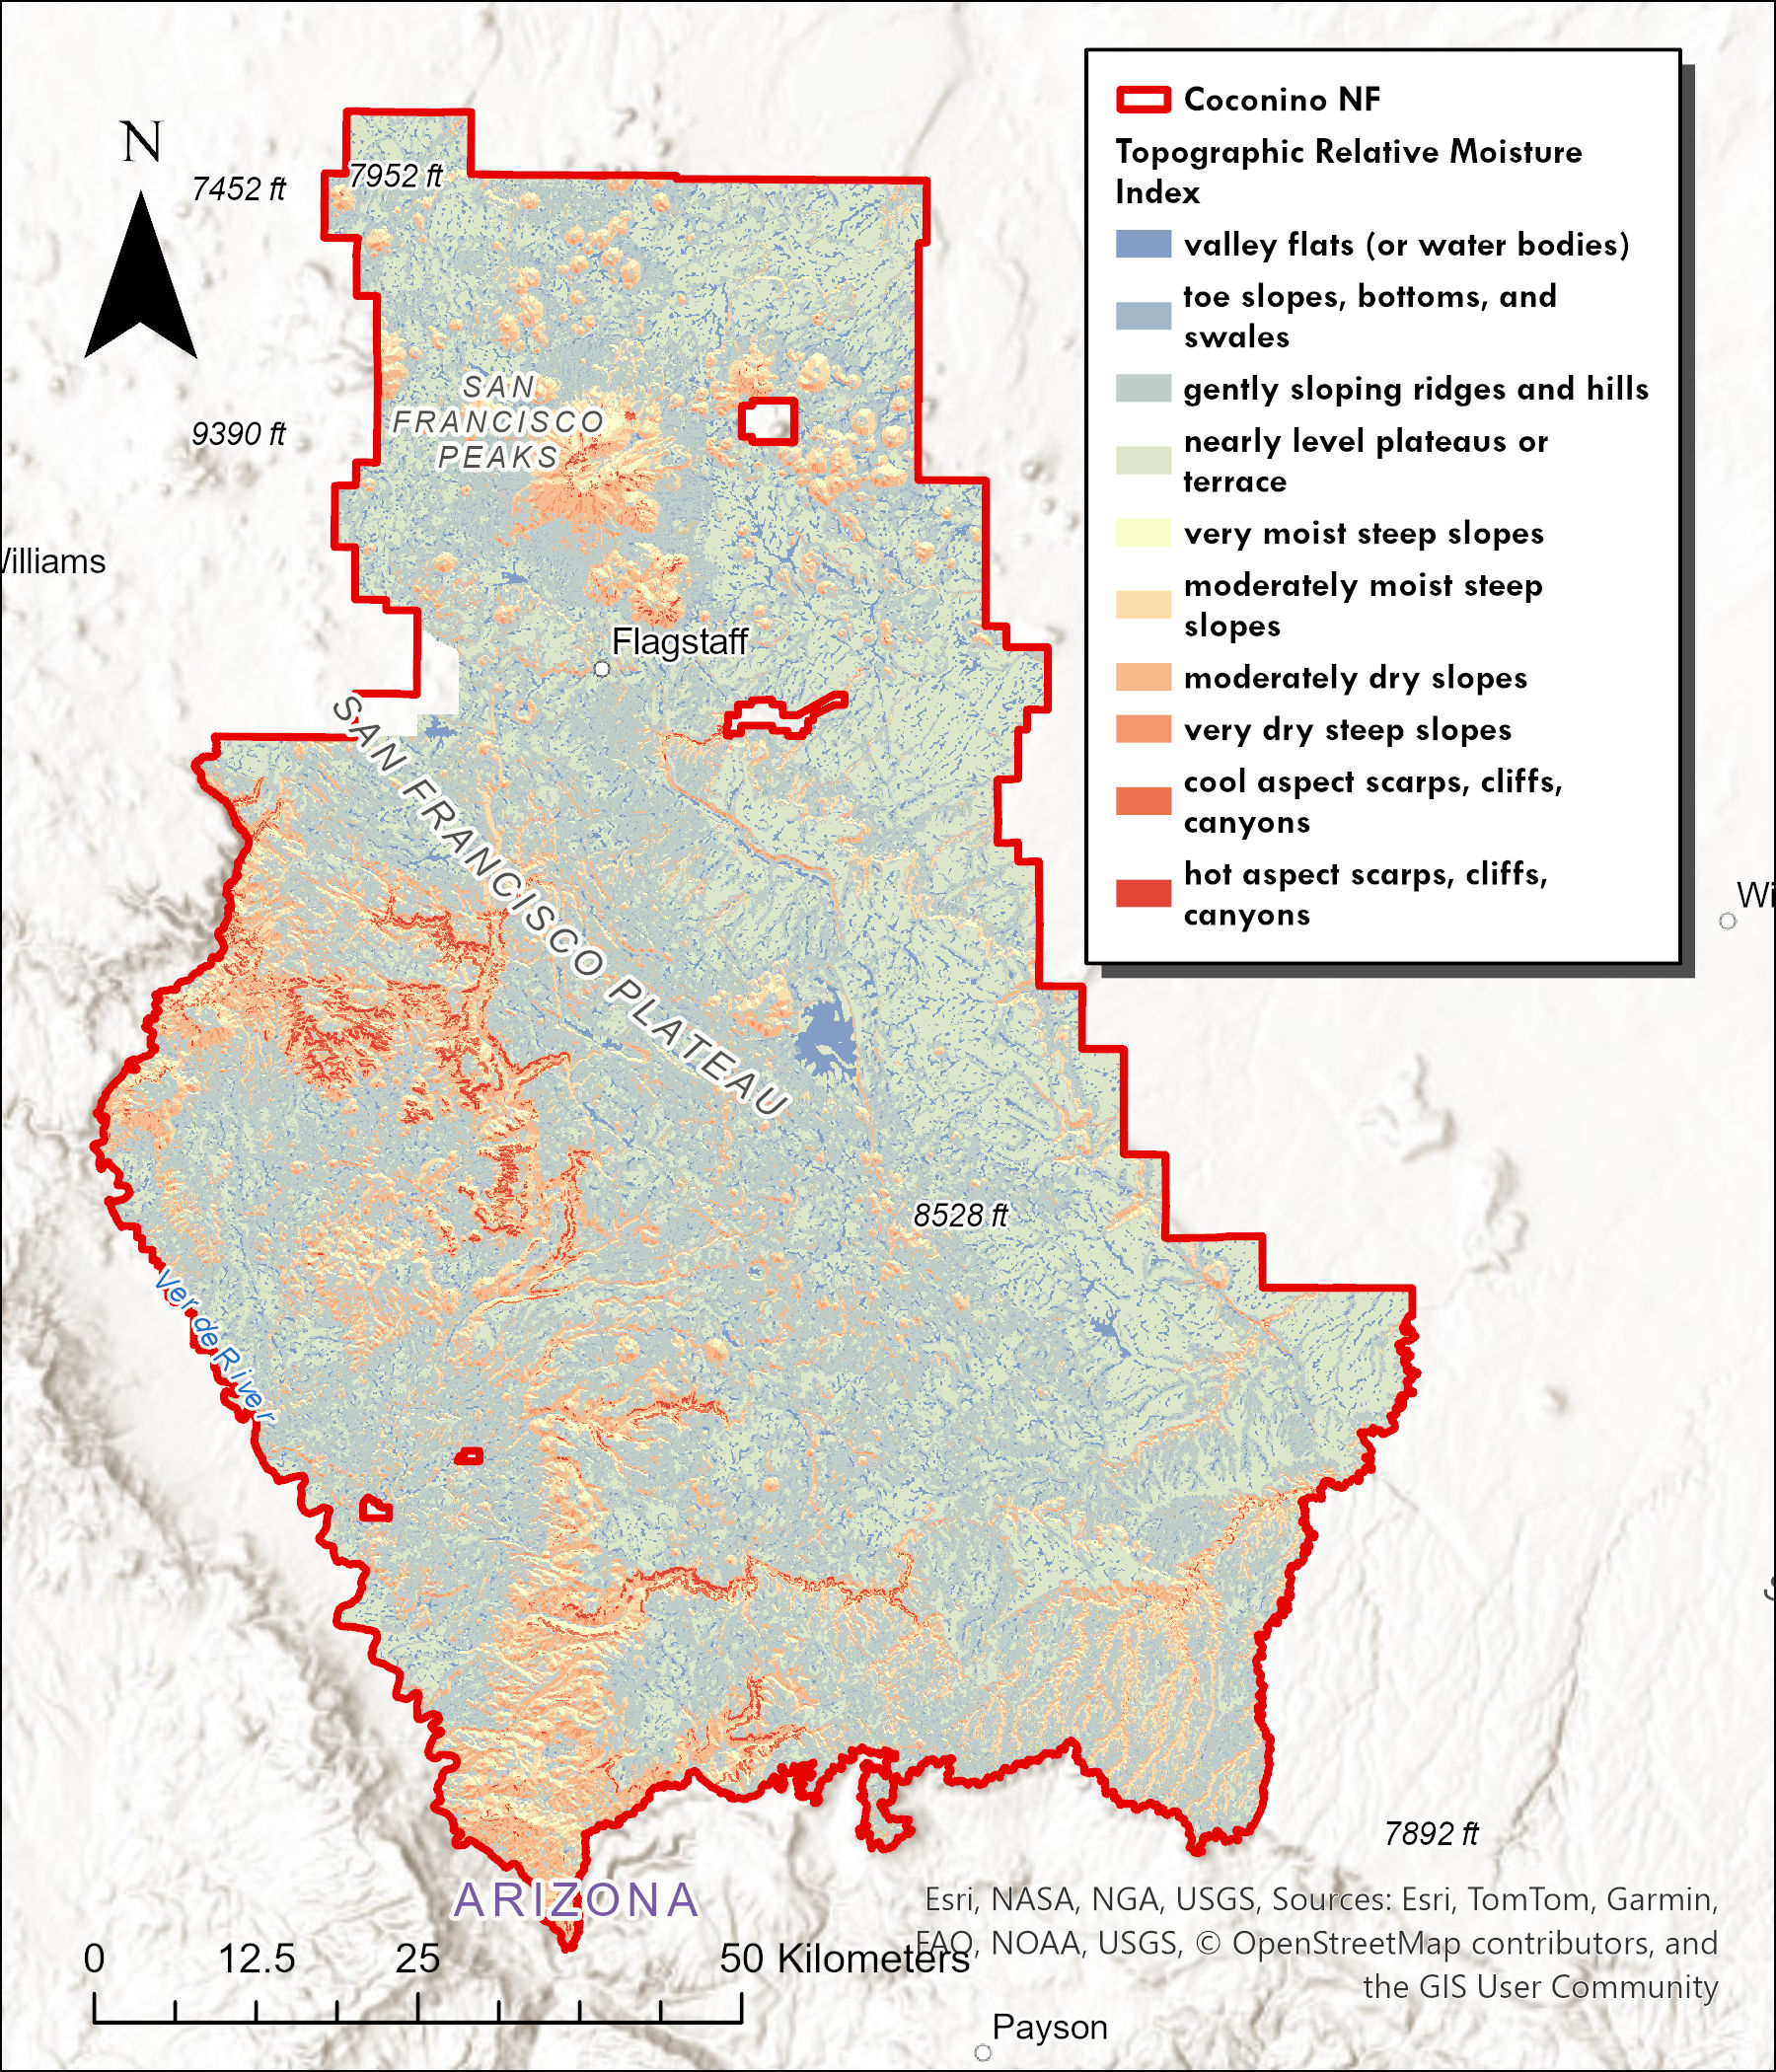
\includegraphics[keepaspectratio]{images/TRMI.jpg}}

}

\caption{Topographic Relative Moisture Index from the Southwest Regional
Gap Analysis (SWReGAP)}

\end{figure}%

\subsubsection{Basal Area}\label{basal-area}

We extracted basal area estimates from the TreeMap 2016
\citep{riley2022} CONUS dataset.

\begin{figure}[H]

{\centering \pandocbounded{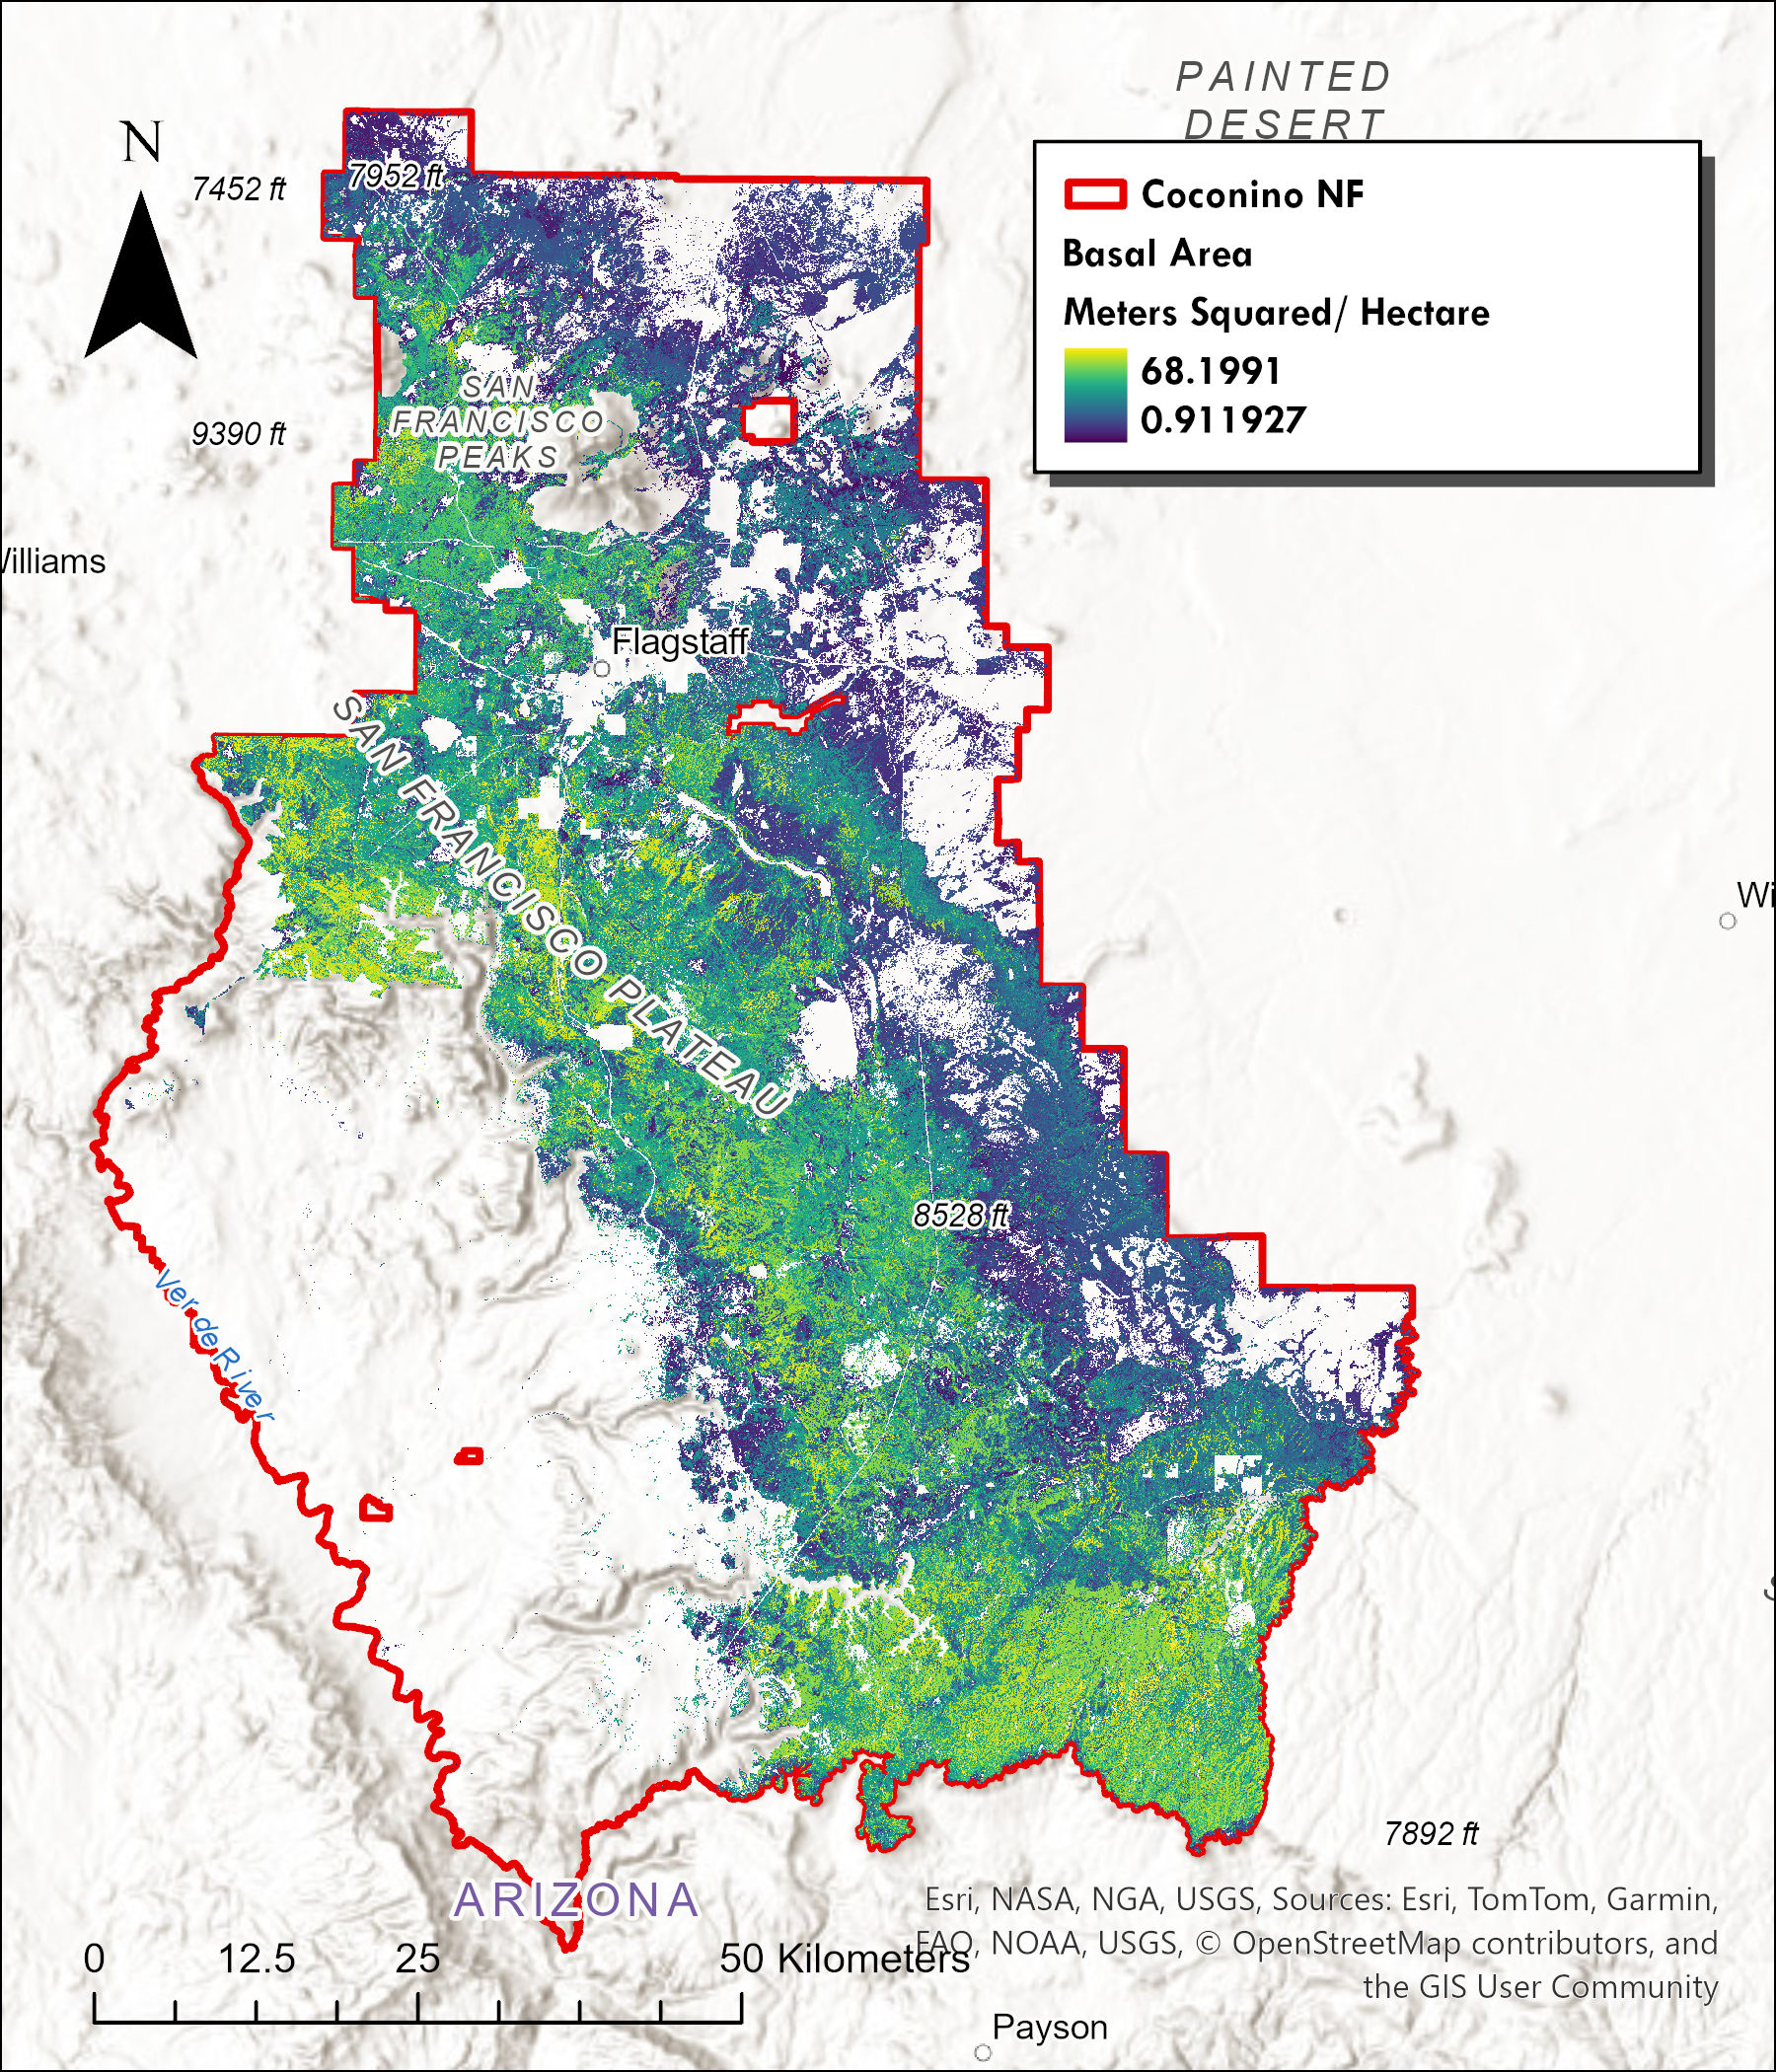
\includegraphics[keepaspectratio]{images/Basal_Area.jpg}}

}

\caption{Basal Area in cubic meters per hectare derived from the 2016
TreeMap dataset.}

\end{figure}%

\subsubsection{Snowfall Dominance}\label{snowfall-dominance}

Ask Patrick Broxton how it was calculated.

\begin{figure}[H]

{\centering \pandocbounded{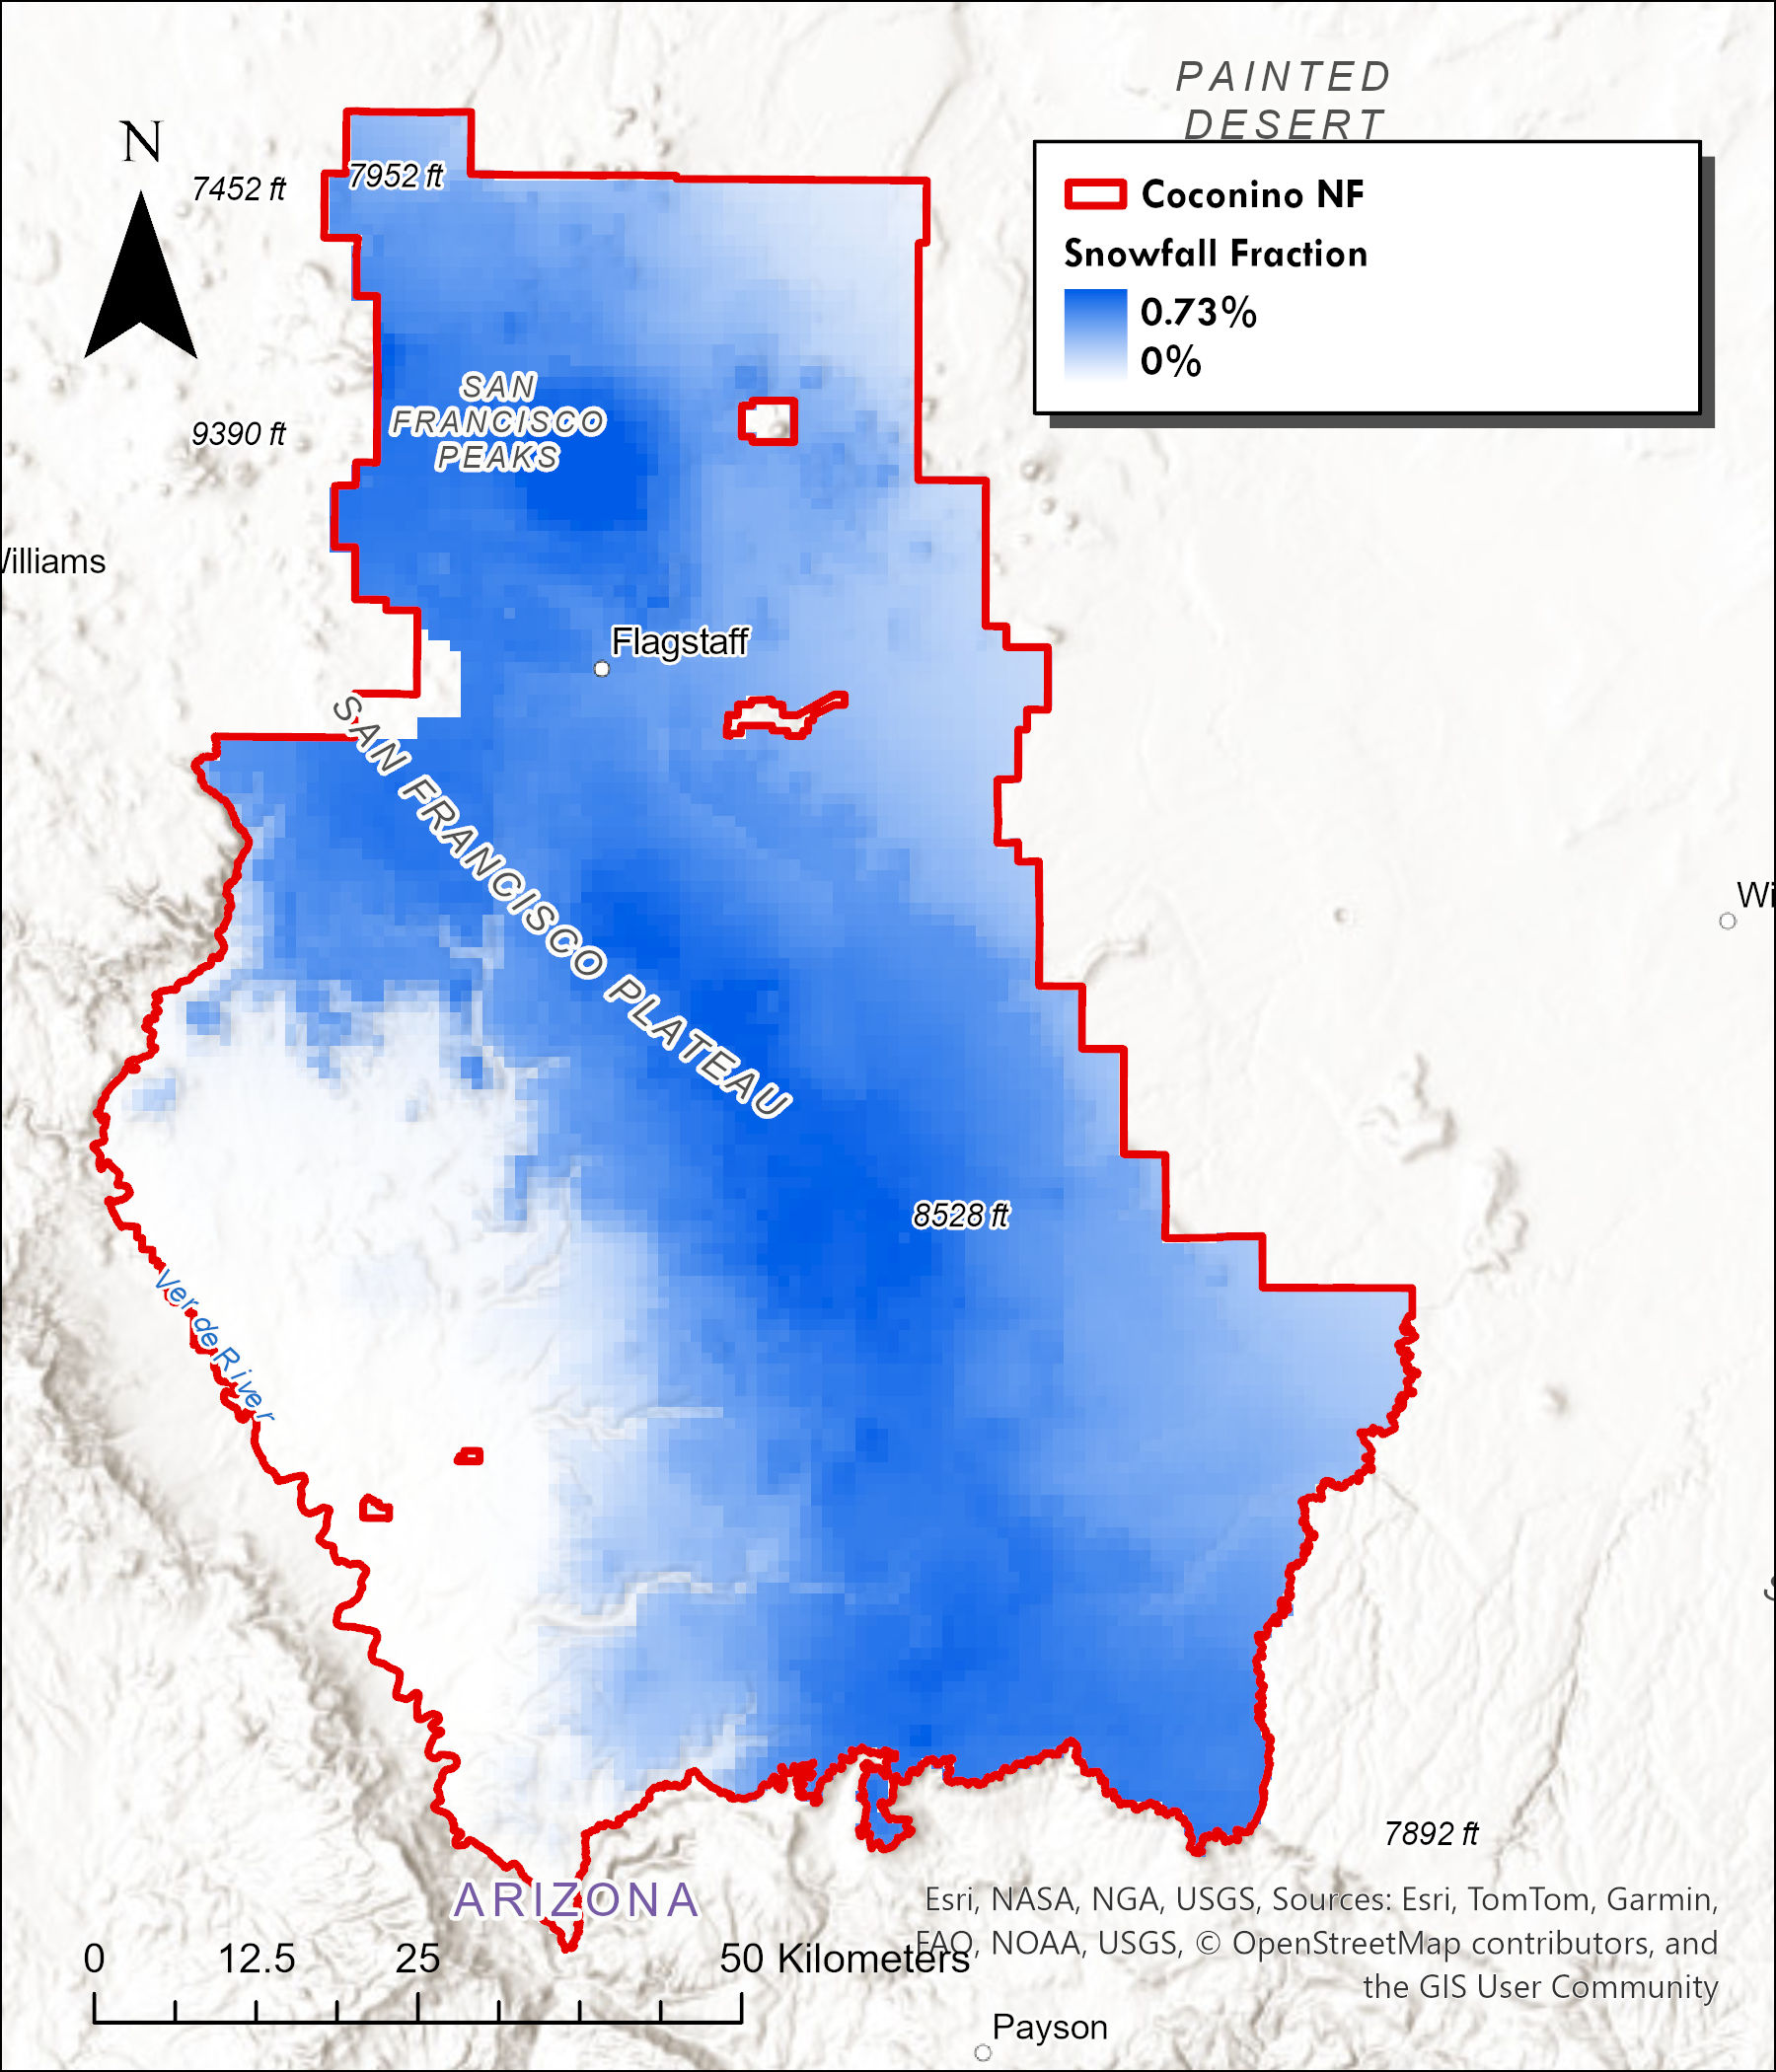
\includegraphics[keepaspectratio]{images/Snowfall Fraction.jpg}}

}

\caption{Percentage of Annual Precipitation that Falls as Snow}

\end{figure}%

\subsubsection{Mean Annual
Precipitation}\label{mean-annual-precipitation}

Utilized AORC Retrospective forcing data for average water year (WY)
precipitation 1991 - 2020

\begin{figure}[H]

{\centering \pandocbounded{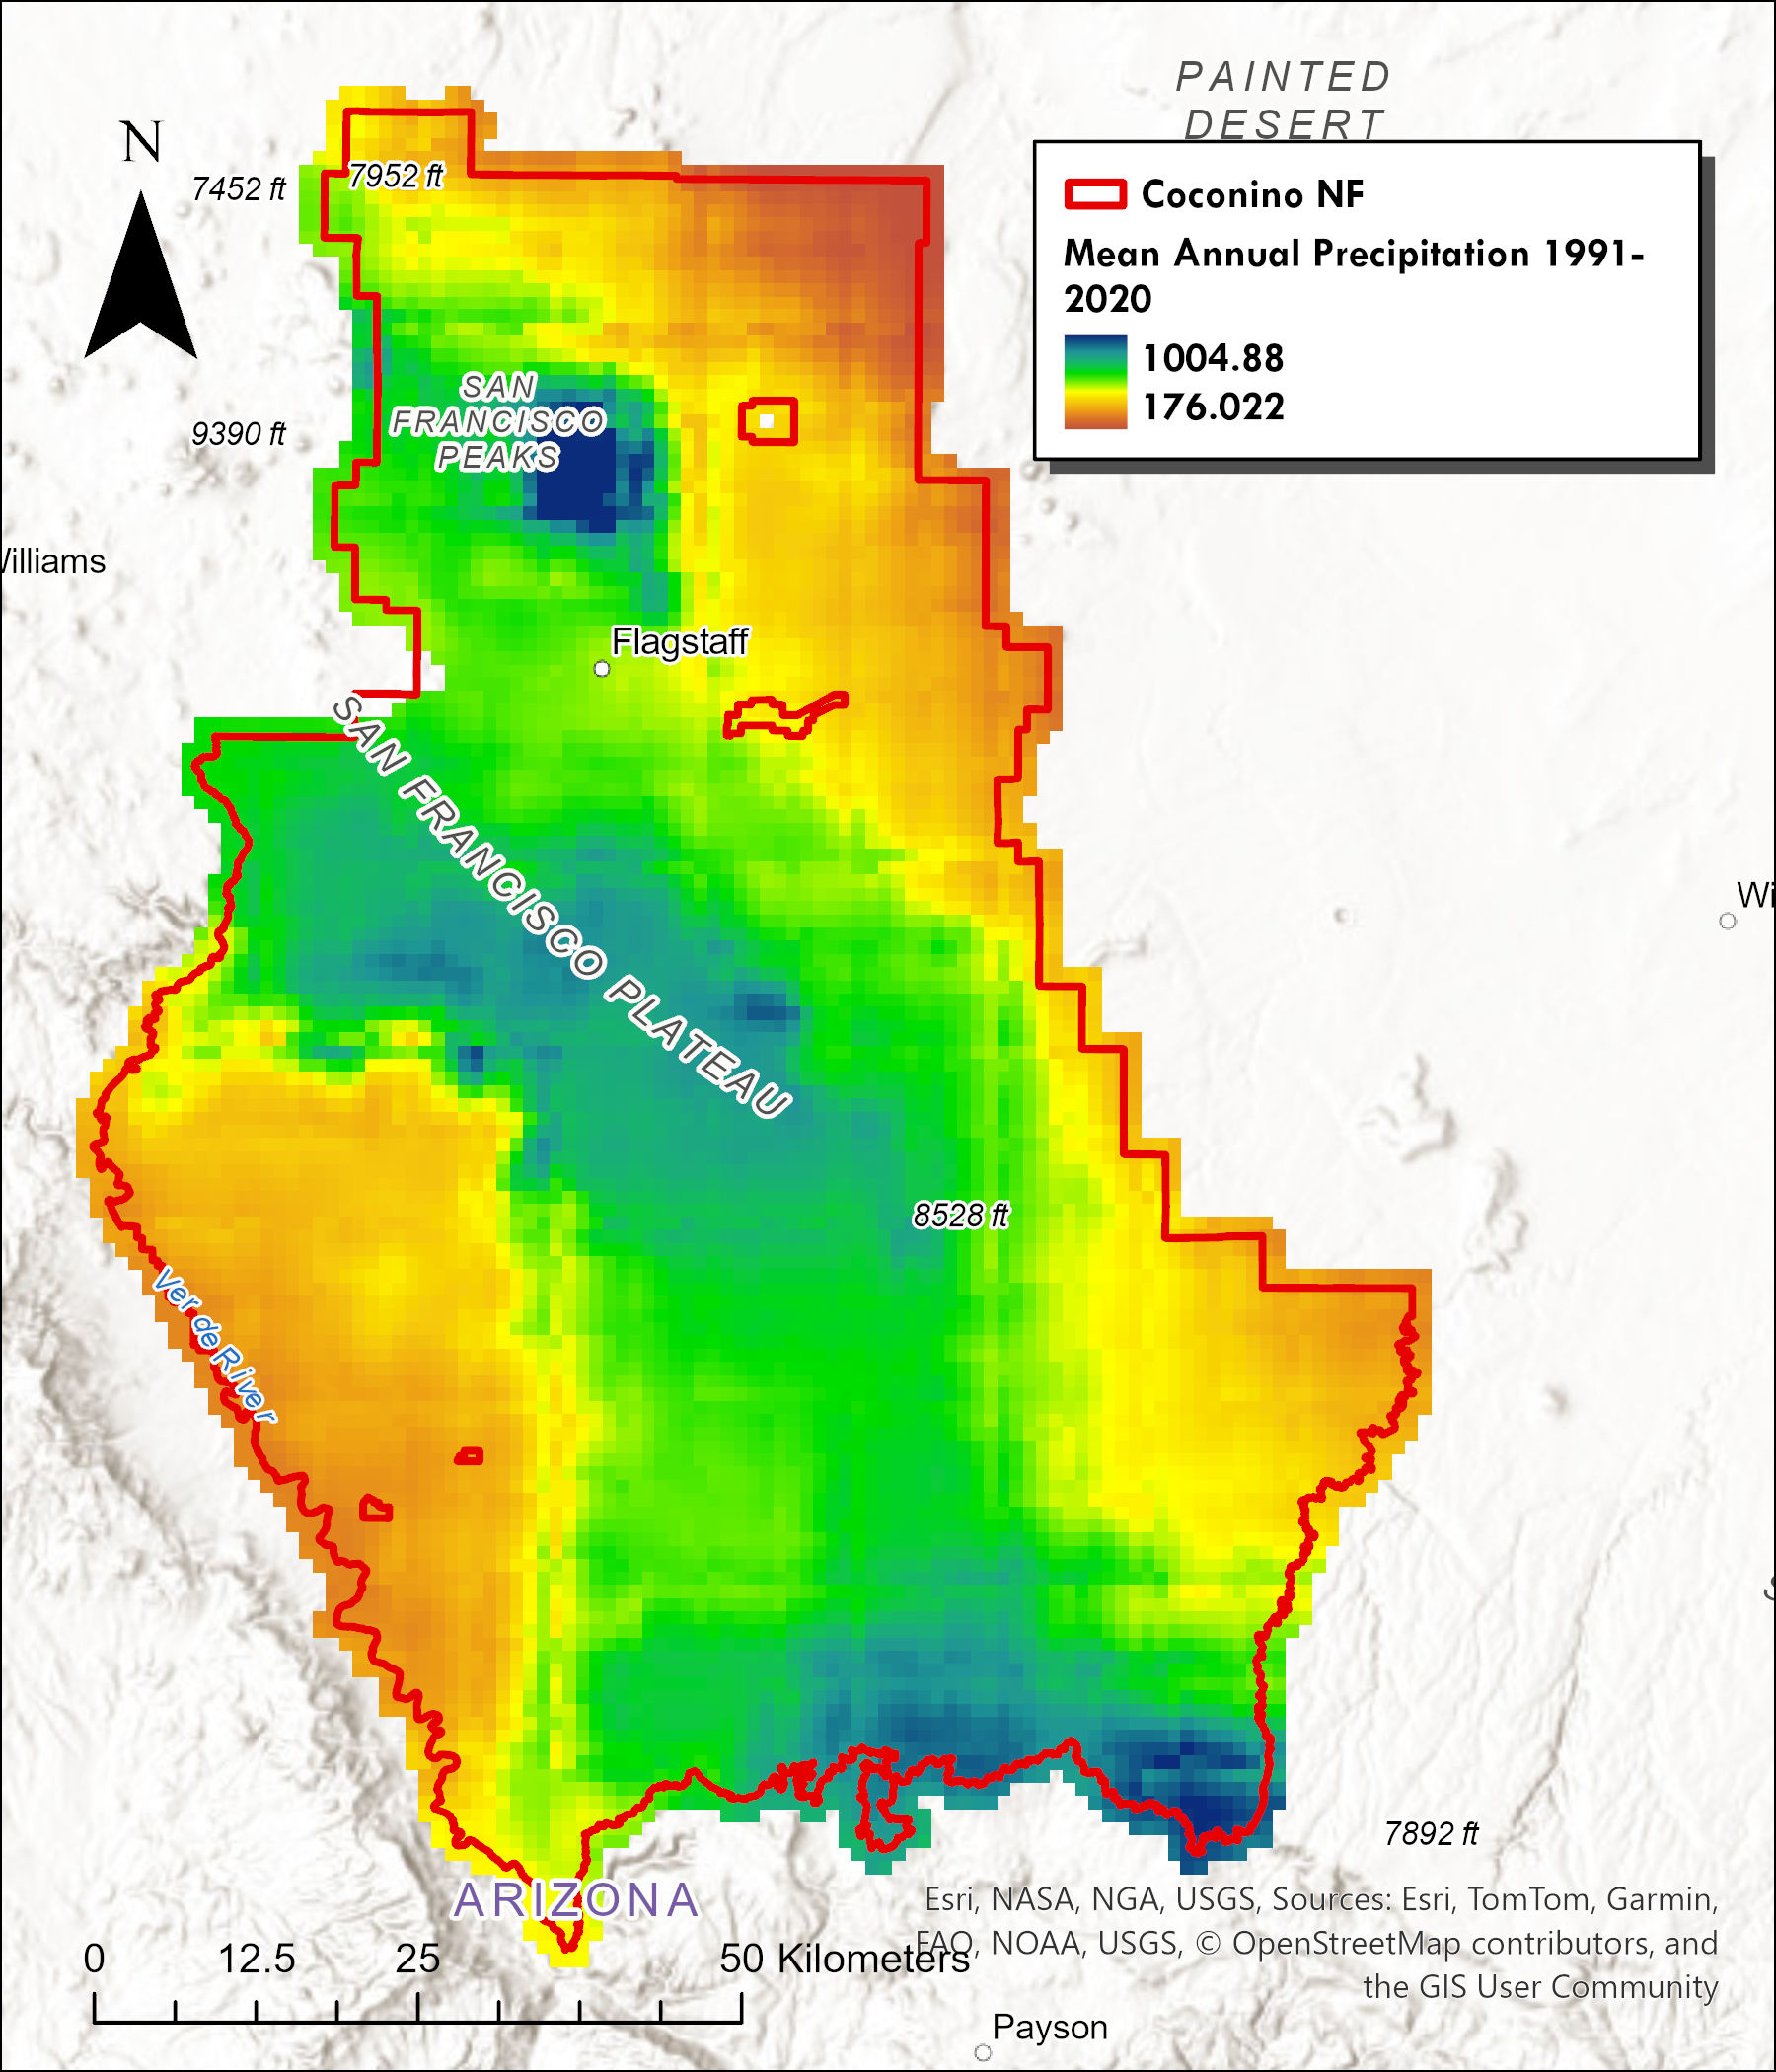
\includegraphics[keepaspectratio]{images/Mean_Annual_Precipitation.jpg}}

}

\caption{Mean Annual Precipitation for years 1991 - 2020}

\end{figure}%

\subsubsection{Subsurface Infiltration
Capacity}\label{subsurface-infiltration-capacity}

We utilized the Global Hydrological Maps of Permeability and Porosity
(GLHYMPS) to estimate subsurface infiltration capacity
\citep{gleeson2014}

\begin{figure}[H]

{\centering \pandocbounded{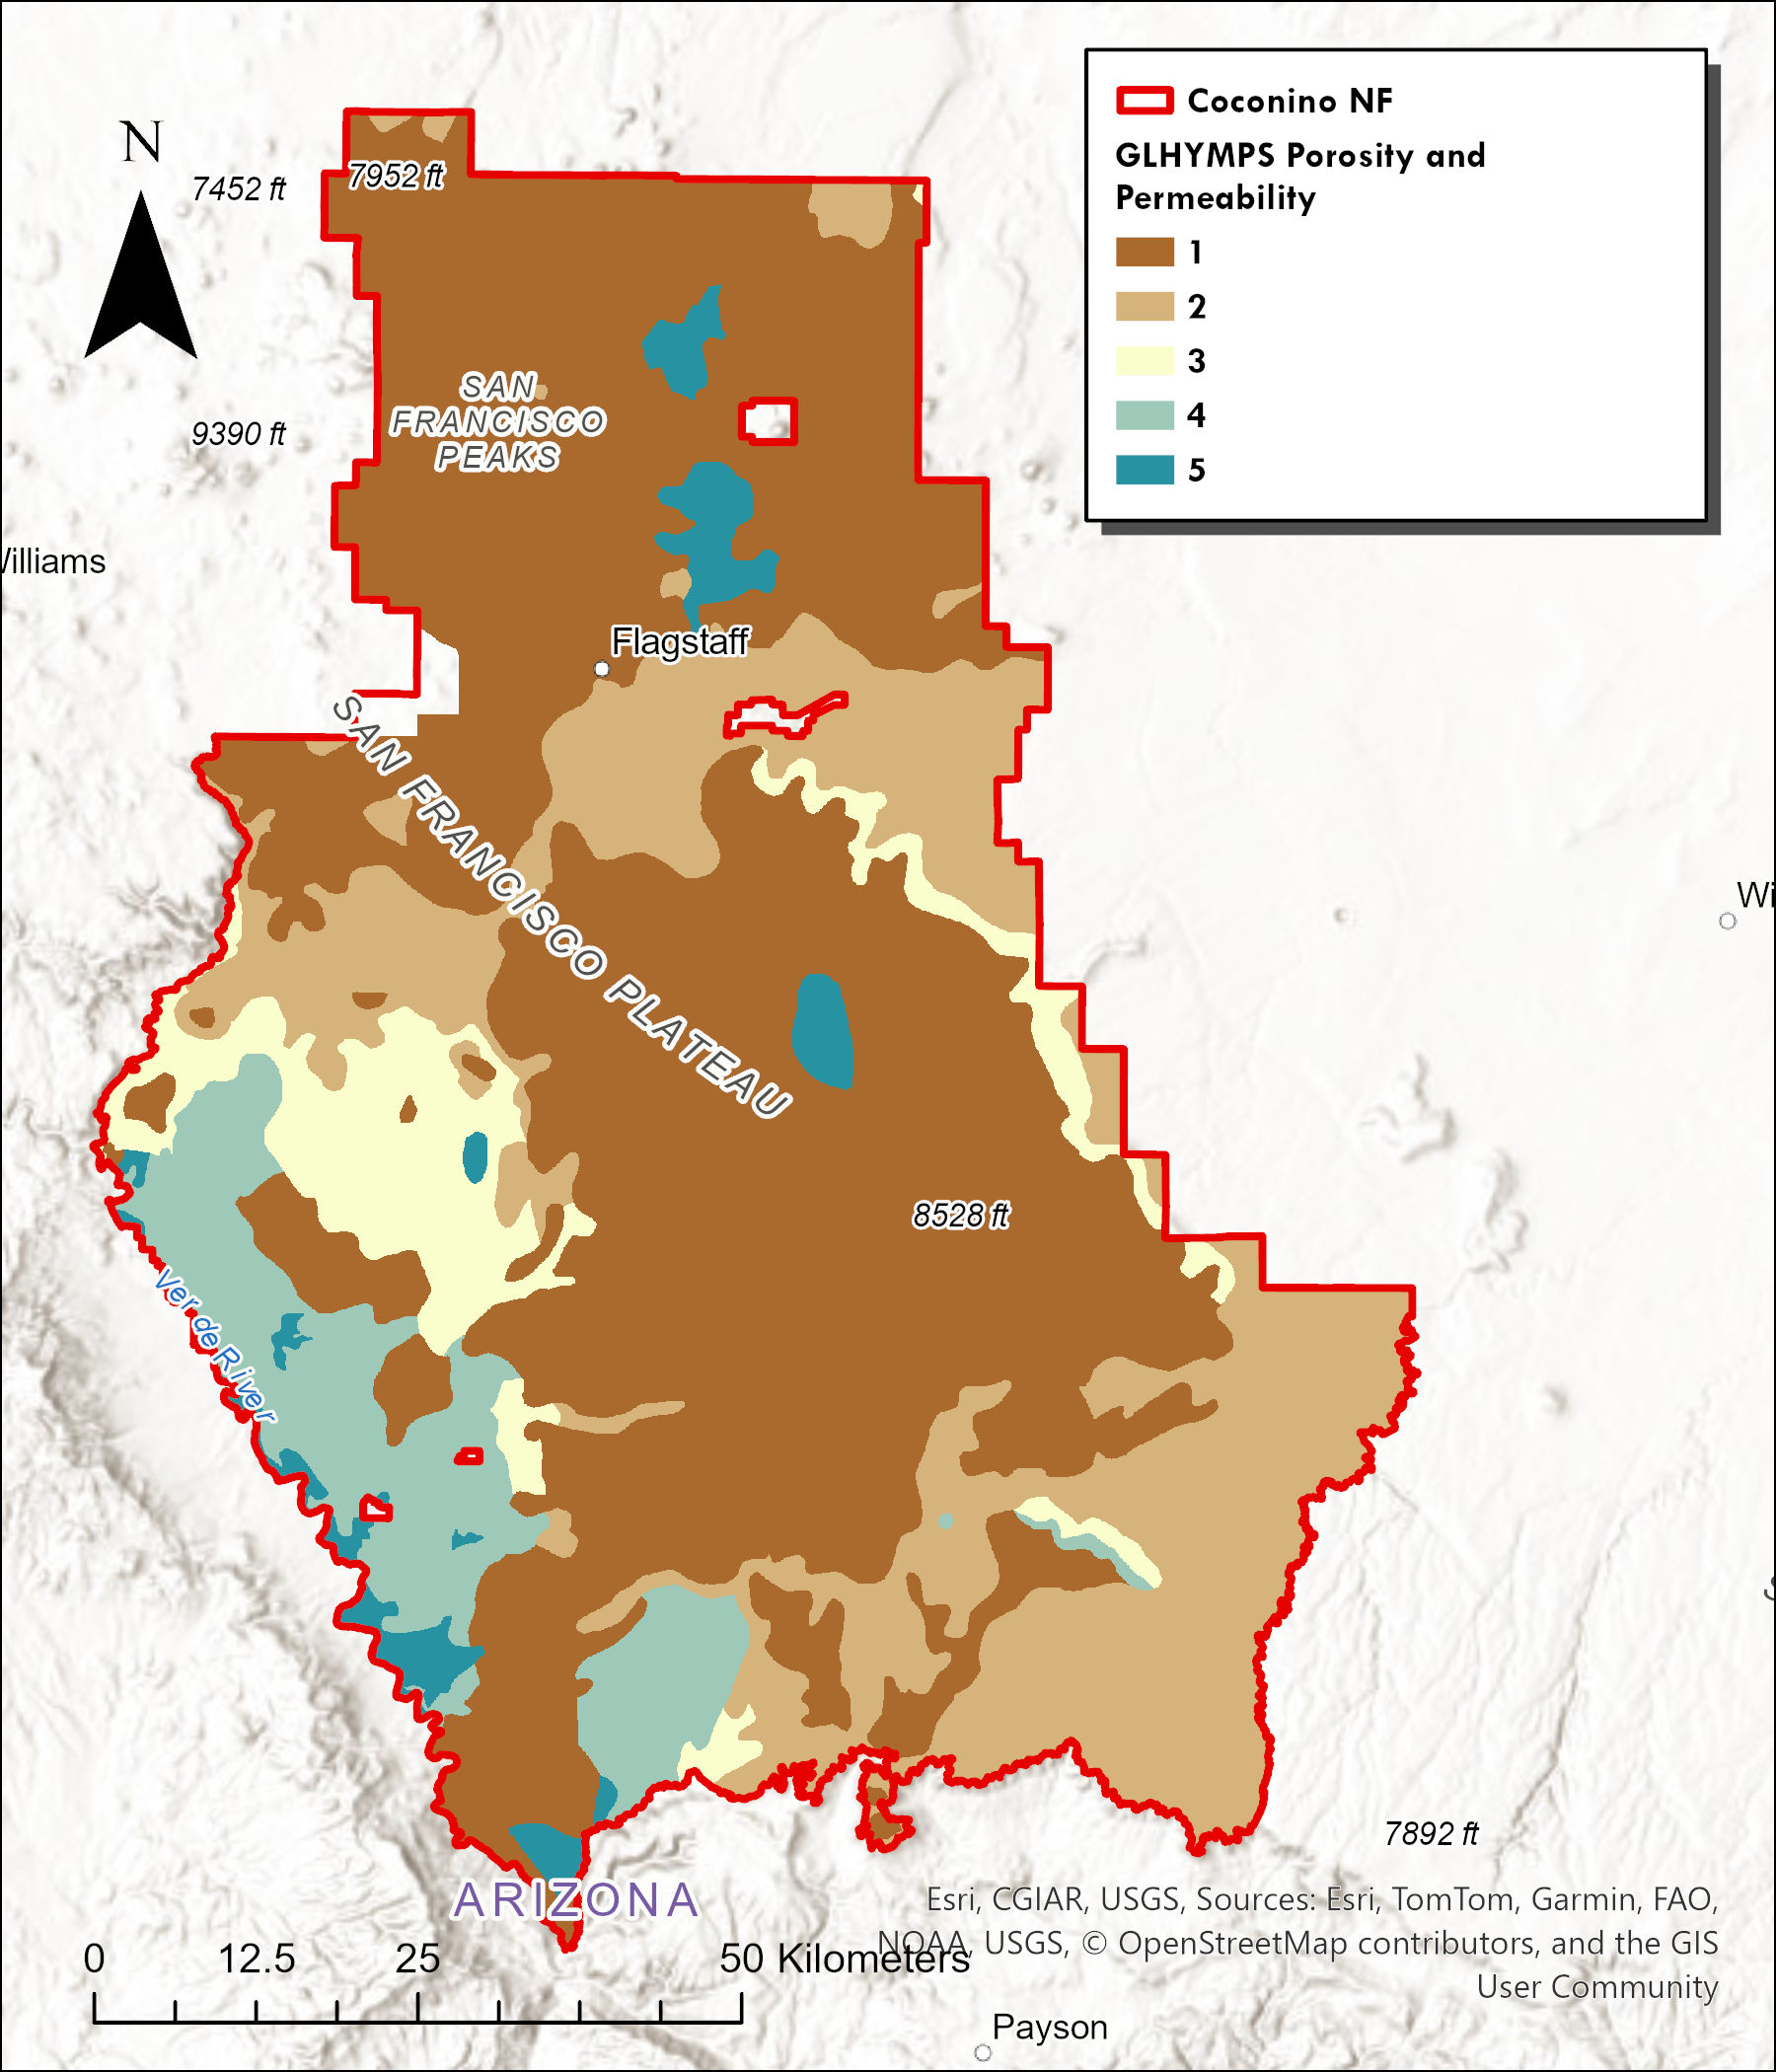
\includegraphics[keepaspectratio]{images/GLHYMPS.jpg}}

}

\caption{Subsurface Infiltration Capacity, a combination of Permeability
and Porosity values from the GLHYMPS dataset (Gleeson et al., 2014).
Higher values (cooler colors) indicate higher infiltration capacity,
while browner colors and lower values indicate lower infiltration
capacity. Keep in mind this does not consider secondary or tertiary
permeability or porosity due to faults, fractures, caves, and conduits.}

\end{figure}%

\subsubsection{Soil Hydrologic Type}\label{soil-hydrologic-type}

Data from gNATSGO was used to estimate the soil's ability to infiltrate
water, we used the Hydrologic Soil Type.

\begin{figure}[H]

{\centering \pandocbounded{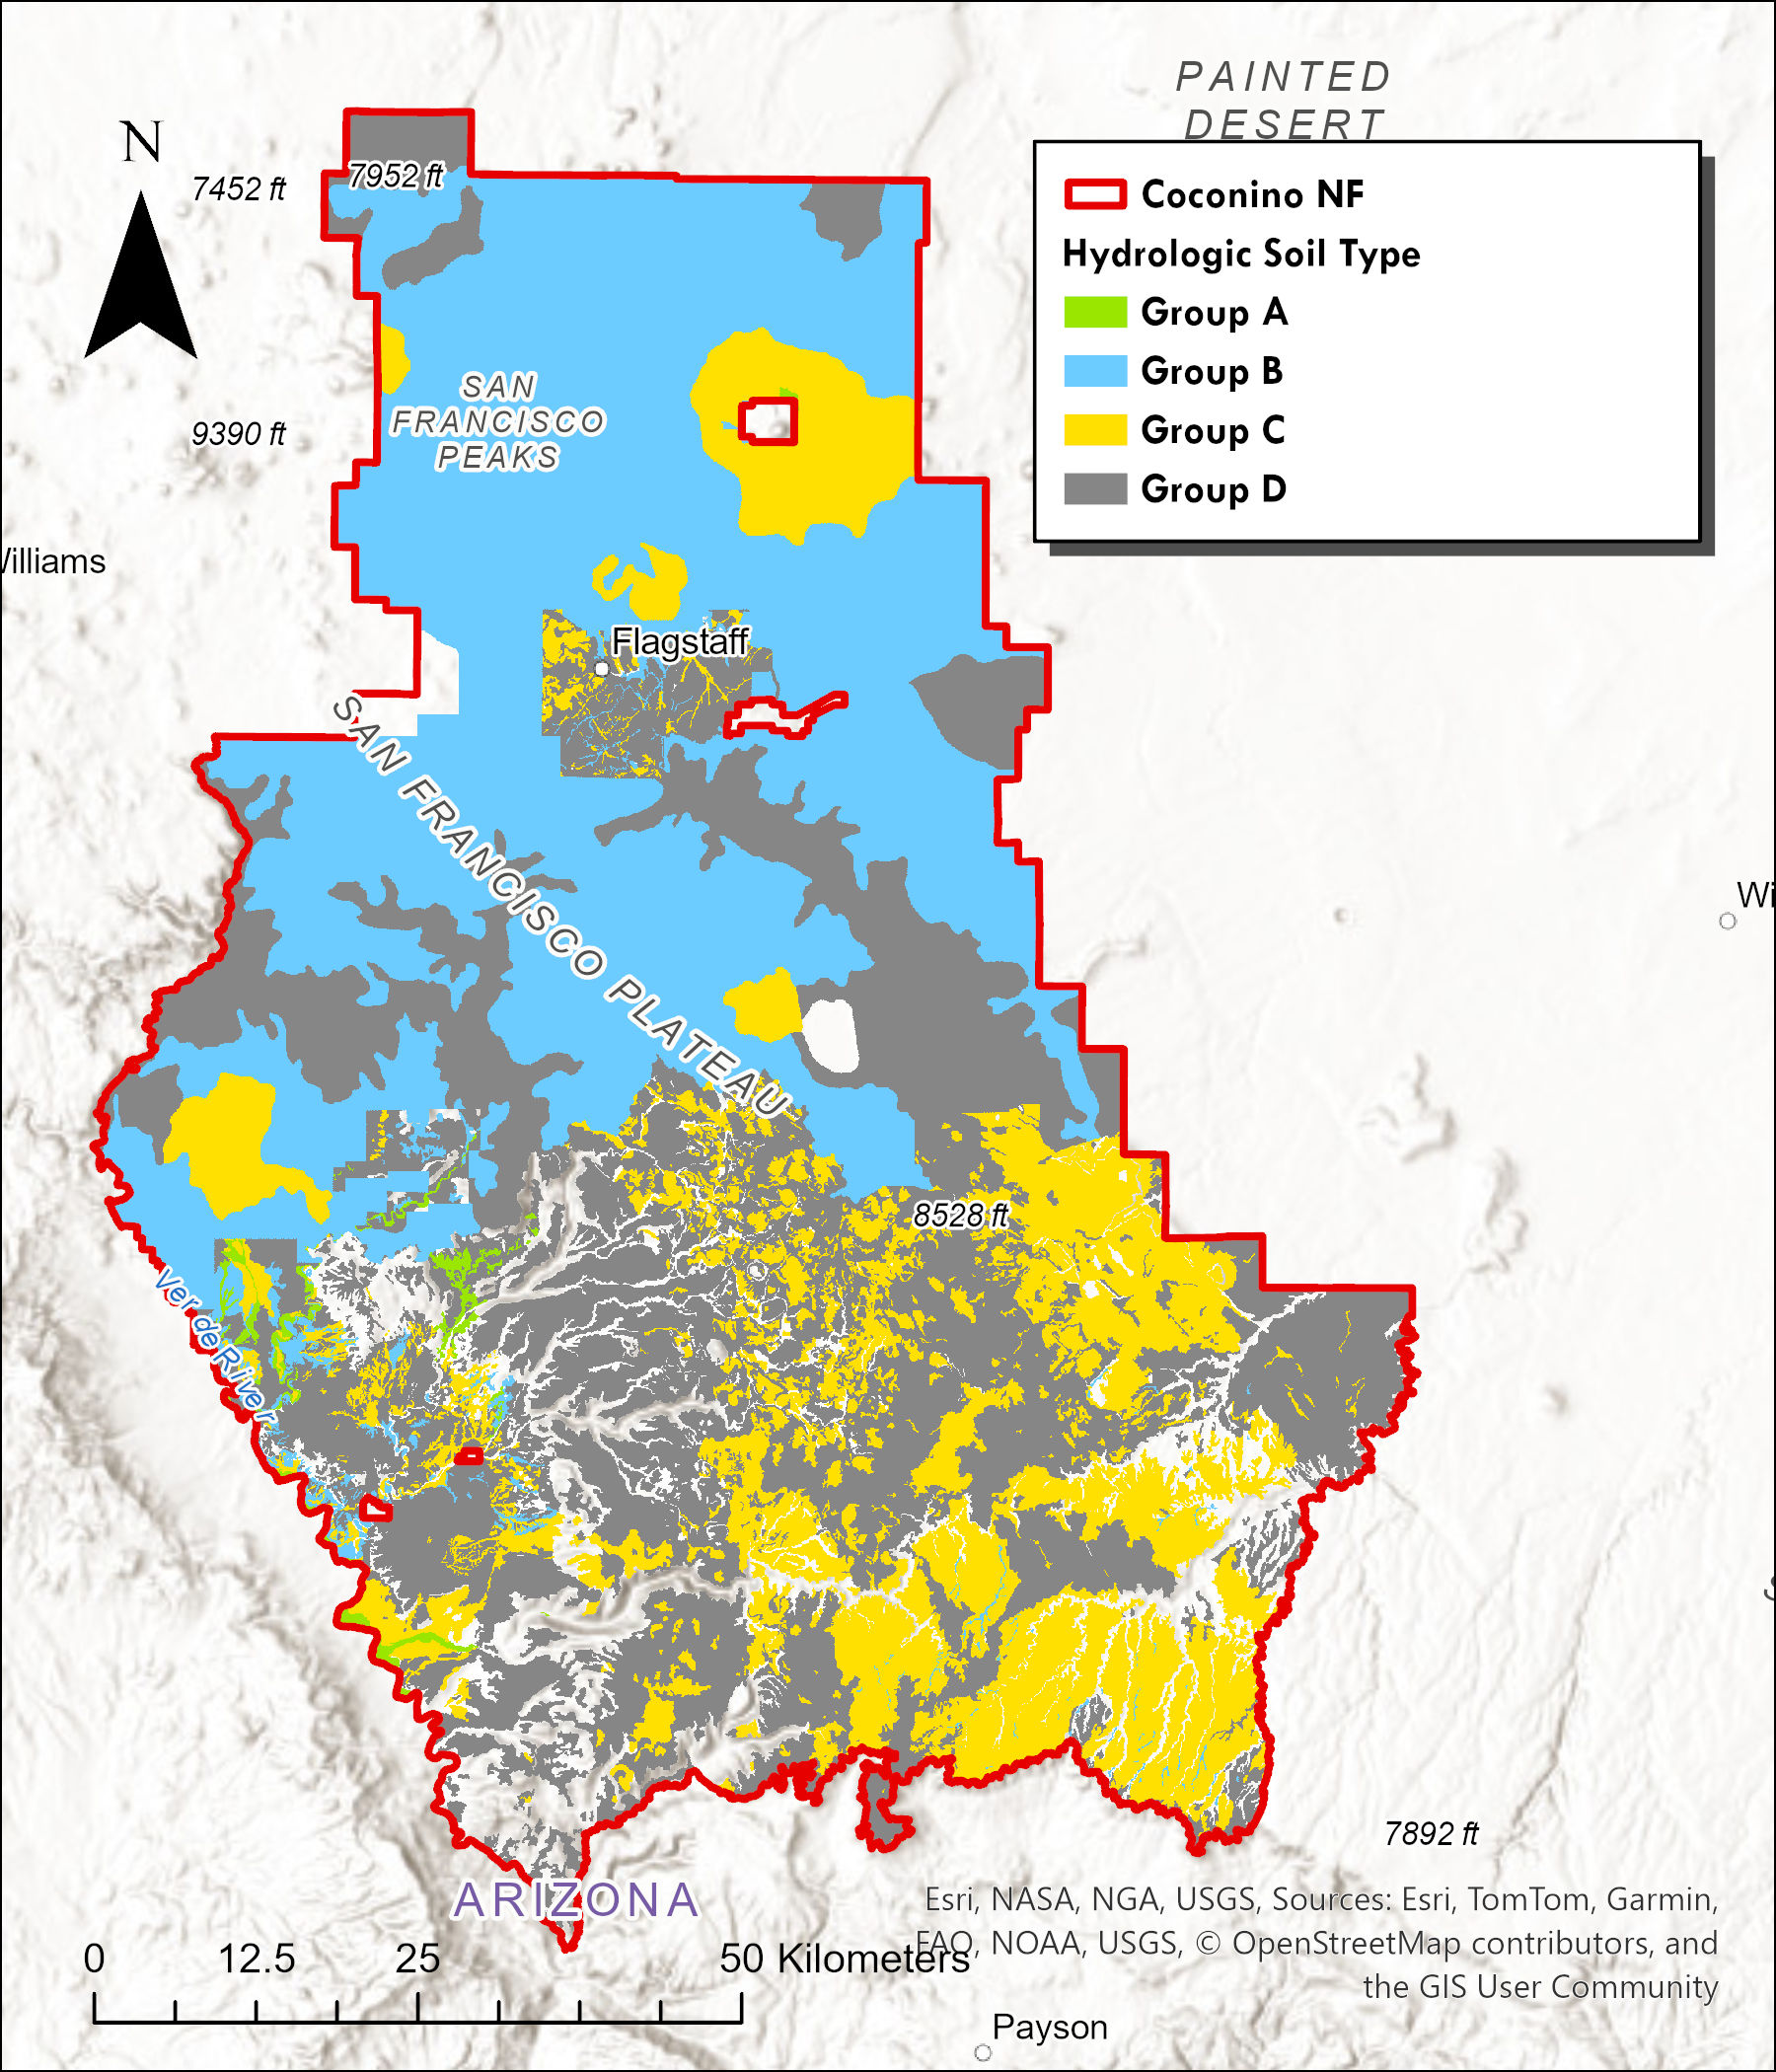
\includegraphics[keepaspectratio]{images/Hydrologic_soil_type.jpg}}

}

\caption{Hydrologic Soil Type from gNATSGO.}

\end{figure}%

\subsubsection{Canopy Cover}\label{canopy-cover}

Canopy Cover was obtained from the 2021 National Land Cover Dataset ,
which provides an estimate of Total Canopy Cover.

\begin{figure}[H]

{\centering \pandocbounded{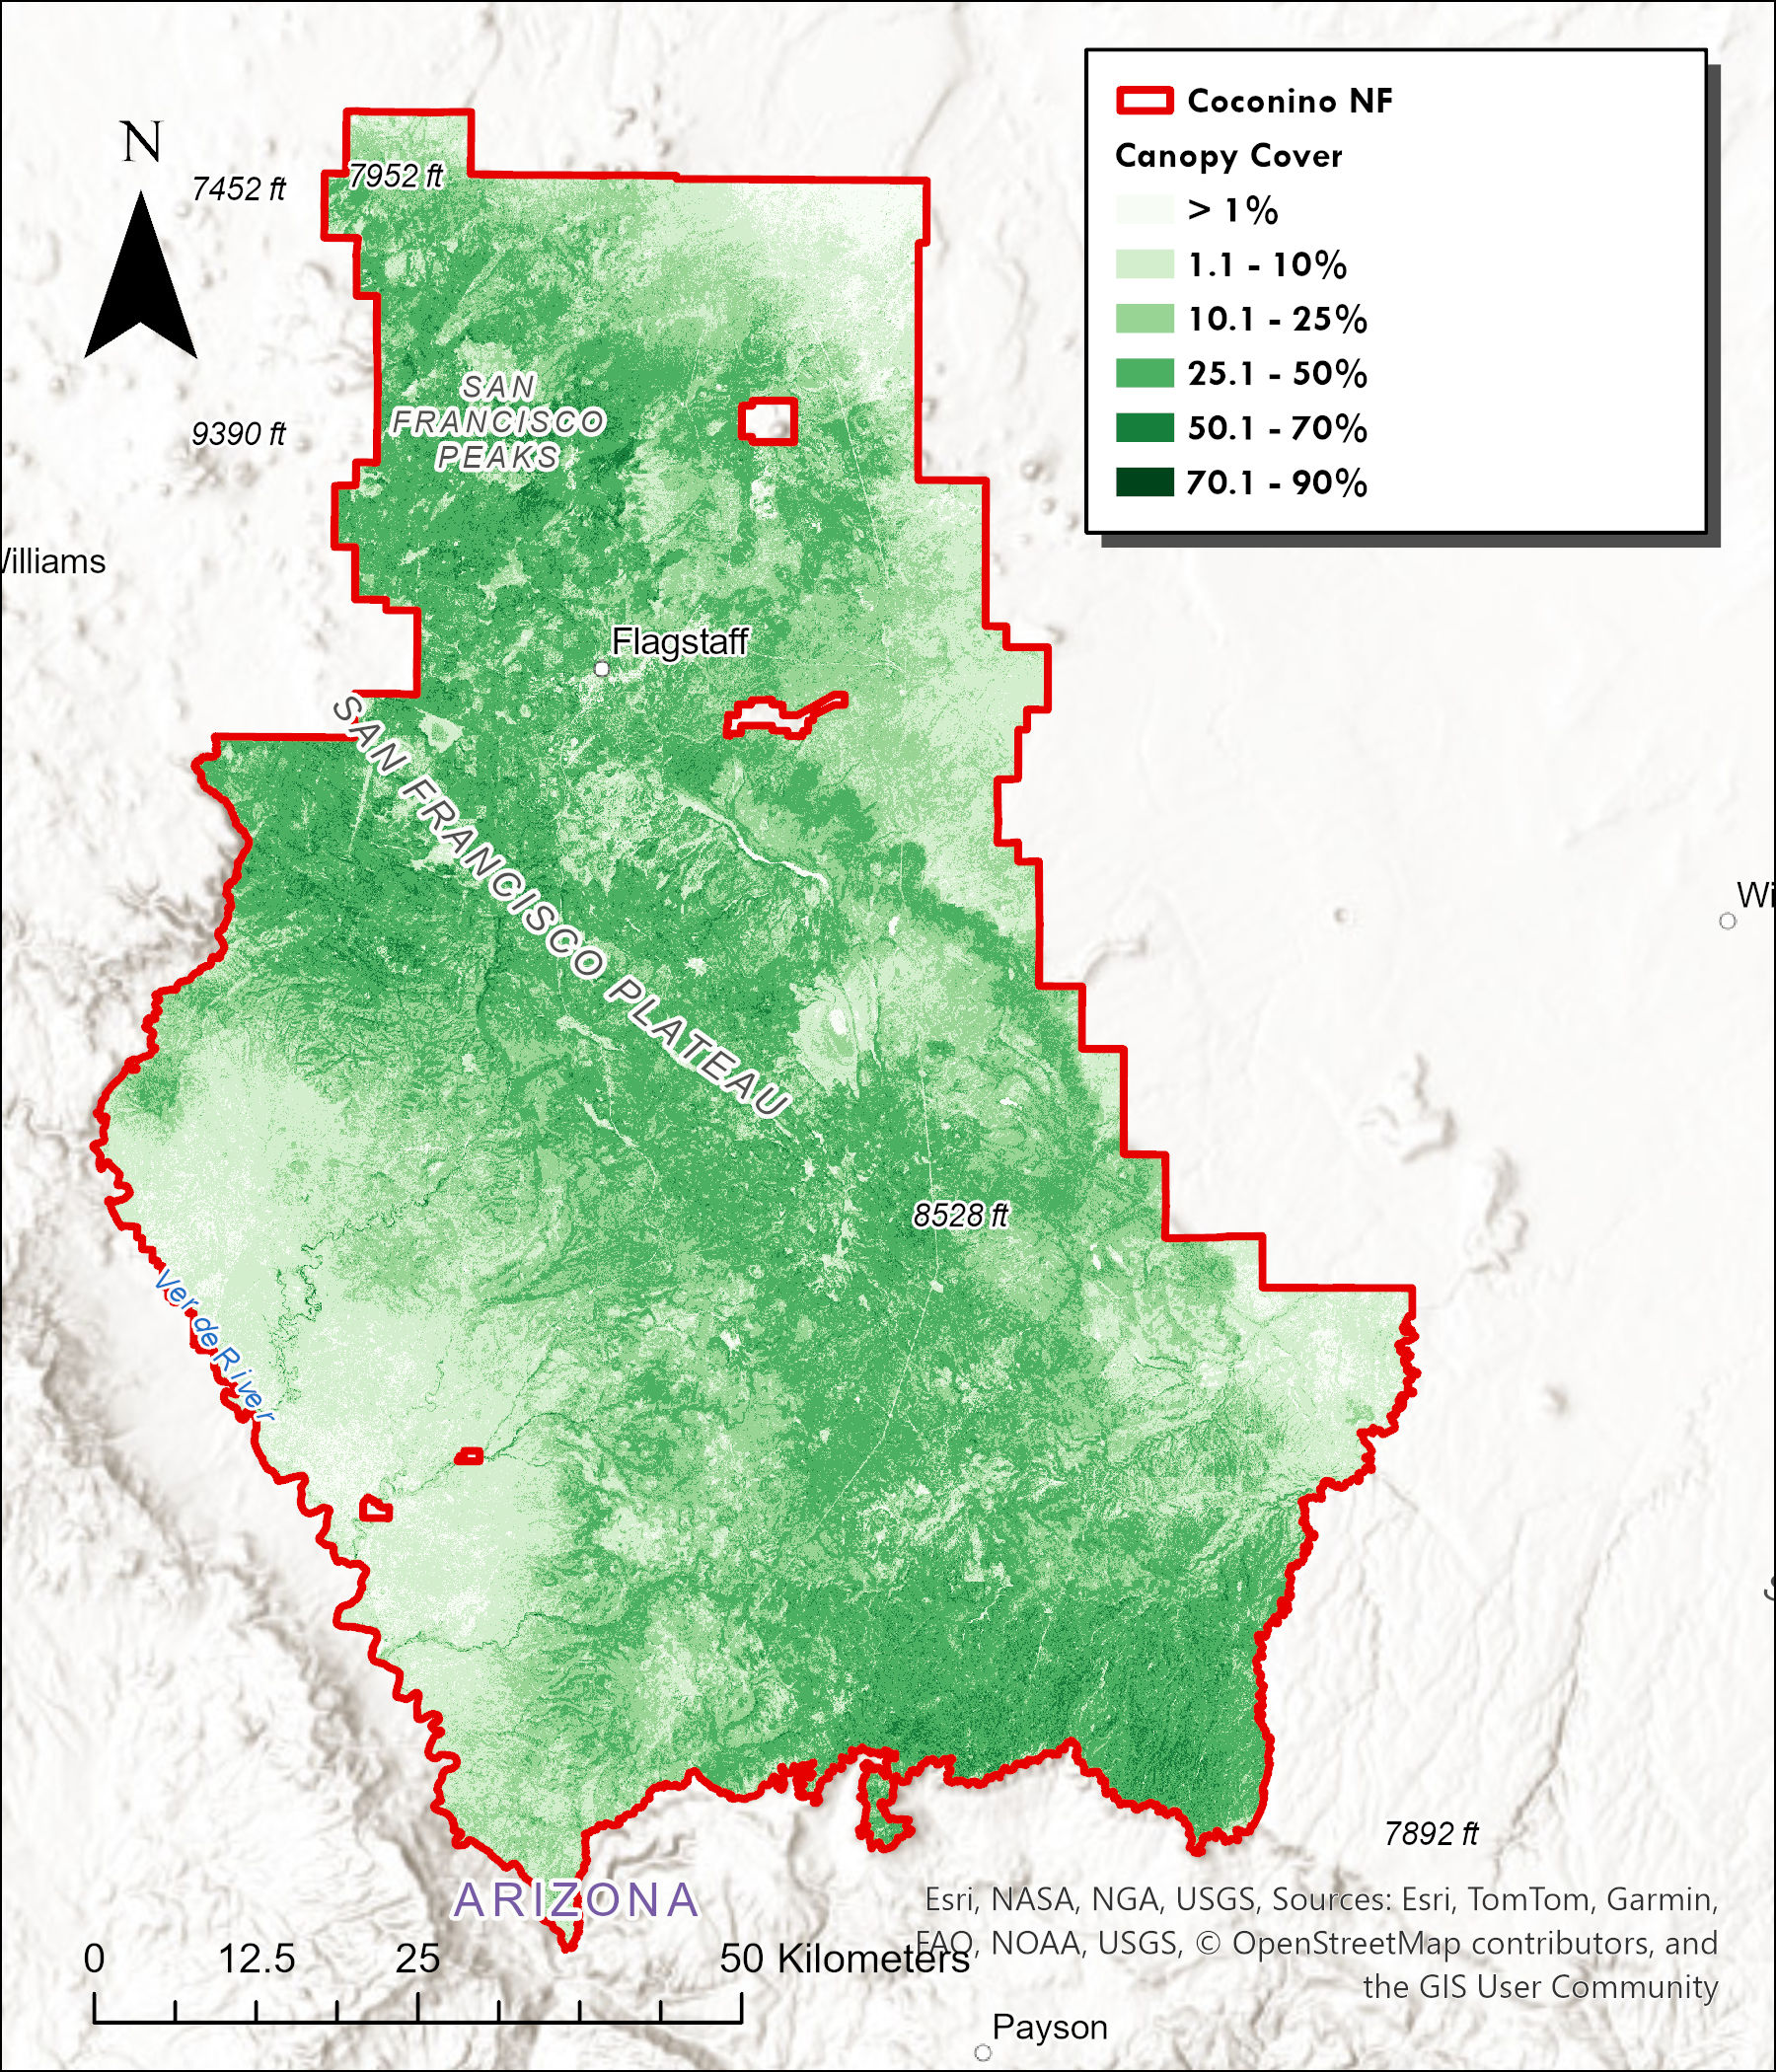
\includegraphics[keepaspectratio]{images/Canopy_Cover.jpg}}

}

\caption{Canopy Cover derived from the NLCD 2021}

\end{figure}%

\subsection{Weighting}\label{weighting}

Pairwise comparisons between each variable were made using the
\href{https://www.inowas.com/tools/t05-gis-mcda/}{INOWAS GIS MCDA tool}

\begin{longtable}[]{@{}ll@{}}
\toprule\noalign{}
Criteria & Weight (\%) \\
\midrule\noalign{}
\endhead
\bottomrule\noalign{}
\endlastfoot
Subsurface Infiltration & 10.12 \\
Canopy Cover & 9.82 \\
Basal Area & 15.06 \\
Topographic Moisture Index & 29.48 \\
Mean annual Precipitation & 10.73 \\
Snowfall Fraction & 14.77 \\
\end{longtable}

\subsection{Model}\label{model}

\begin{figure}[H]

{\centering \pandocbounded{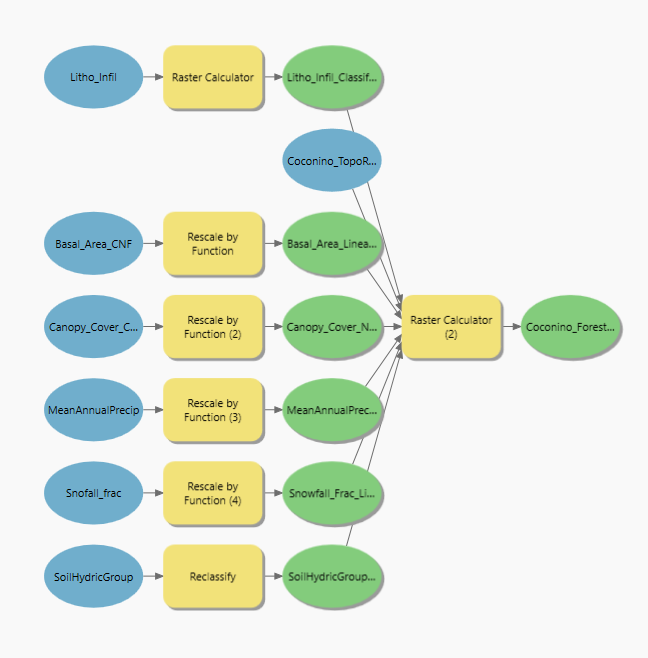
\includegraphics[keepaspectratio]{images/ArcGIS_Model_builder.png}}

}

\caption{This is a diagram of the Suitability model (maybe we can make a
prettier version)}

\end{figure}%

\section{Results}\label{results}

After excluding wilderness areas, areas receiving less than 500 \(mm\)
maximum annual precipitaiton and non-compatible land uses, there is
about 480,000 hectares that were evaluated for suitability for thinning
to enhance recharge. About 95,000 ha have suitability values of 5 or
greater, about 12,000 ha have suitability values of 6 or greater, and 65
ha with suitability values greater than 7. Leaving about 384,000 ha with
suitability scores less than 5. This does not mean recharge will not be
enhanced by thinning in these areas but treatments are less likely to
enhance recharge in those areas.

\begin{figure}[H]

{\centering \pandocbounded{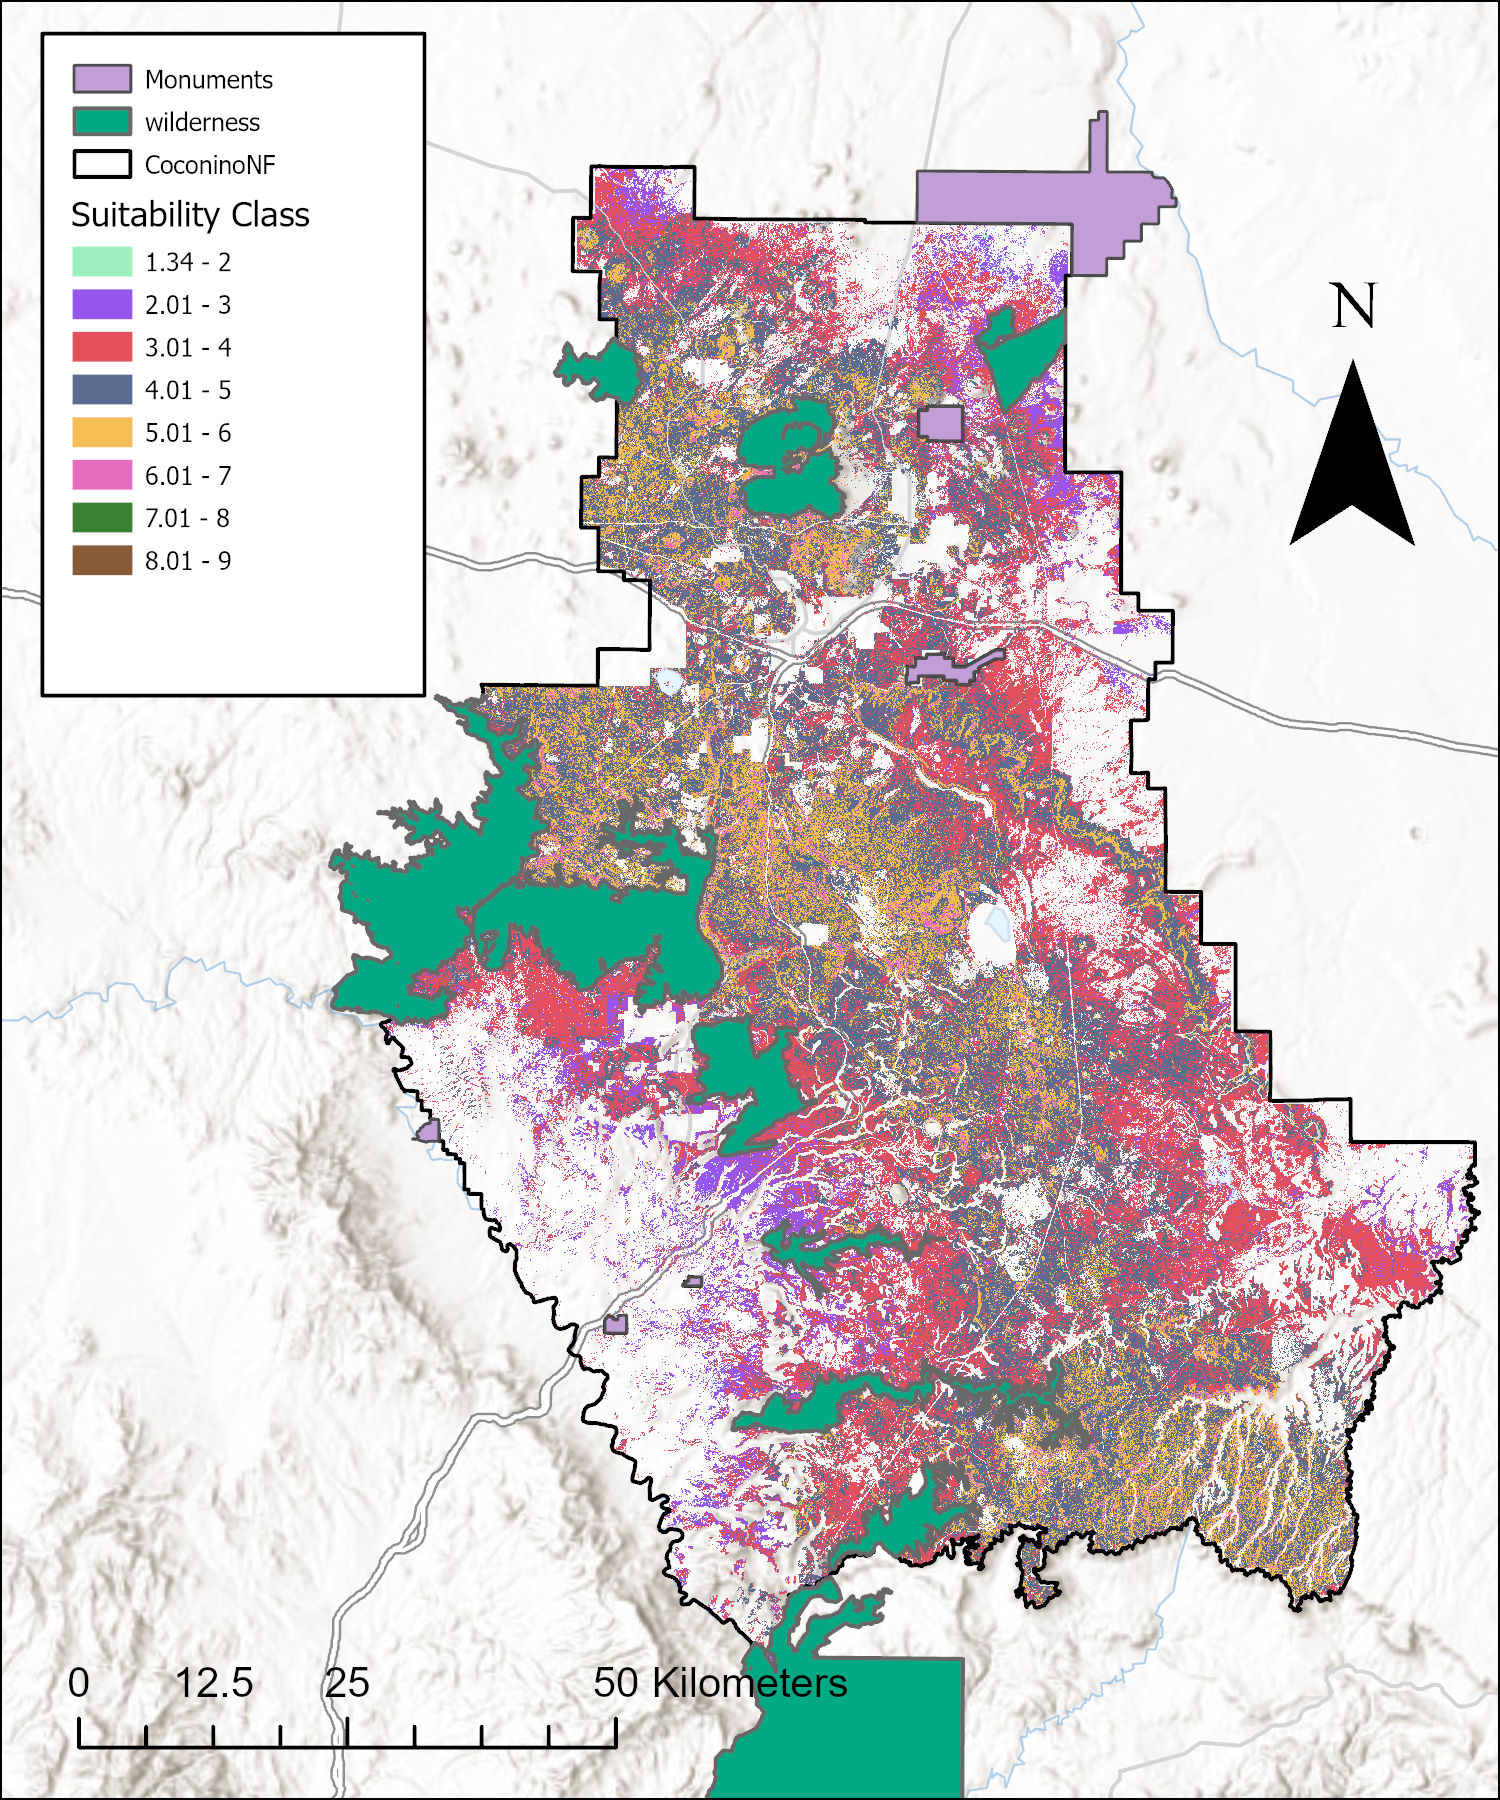
\includegraphics[keepaspectratio]{images/Suitability_map_travis.jpg}}

}

\caption{Suitability Map for Thinning to Enhance Groundwater Recharge}

\end{figure}%

\section{Conclusion}\label{conclusion}

\begin{itemize}
\tightlist
\item
  There are significant portions of the Coconino forest that if thinned,
  are likely to enhance groundwater recharge, however these are not the
  only benefits. While this study was aimed at maximizing recharge,
  these same areas are also likely to reduce wildfire risk and improve
  watershed function enhancing other hydrologic services.
\end{itemize}

\section{Discussion}\label{discussion}

\begin{itemize}
\item
  novel application of MCDA for mapping areas where forest thinning may
  enhance groundwater recharge.
\item
  Could be adapted to other semi-arid forested
\item
  The forest service has a mandate to manage for multiple uses, however
  groundwater recharge is not currently a use that is explicitly managed
  for. However, analyses like these can help identify areas that could
  be managed with aquifer recharge in mind.
\end{itemize}

\subsection{Future Work}\label{future-work}

\begin{itemize}
\item
  Adjusting the suitability map to capture secondary and tertiary
  permeability and porosity in areas underlain by karst
\item
  improved hydrologeolic mapping could improve this process, using
  higher-resolution data for subsurface infiltration rate.
\item
  the soil criteria could be refined by mapping soil Hydraulic
  conductivity and field capacity rather than just using soil types A -
  D providing more detail.
\item
  could be validated with modeling
\item
  Paired watershed studies such as those planned in the Lake Mary
  Watershed with groundwater monitoring can be used to validate and fine
  tune model weighting and decision rules between criteria.
\item
  this methodology could be used across the 2.6 million acres of
  Ponderosa Pine forest in Arizona and New mexico
\item
  State-wide and regional geologic mapping in Arizona is currently only
  at the 1:500,000 scale, more detailed data could improve this type of
  suitability mapping.
\end{itemize}

\section{Acknowledgments}\label{acknowledgments}

Phasellus interdum tincidunt ex, a euismod massa pulvinar at. Ut
fringilla ut nisi nec volutpat. Morbi imperdiet congue tincidunt.
Vivamus eget rutrum purus. Etiam et pretium justo. Donec et egestas sem.
Donec molestie ex sit amet viverra egestas. Nullam justo nulla,
fringilla at iaculis in, posuere non mauris. Ut eget imperdiet elit.

\section{Open research}\label{open-research}

Phasellus interdum tincidunt ex, a euismod massa pulvinar at. Ut
fringilla ut nisi nec volutpat. Morbi imperdiet congue tincidunt.
Vivamus eget rutrum purus. Etiam et pretium justo. Donec et egestas sem.
Donec molestie ex sit amet viverra egestas. Nullam justo nulla,
fringilla at iaculis in, posuere non mauris. Ut eget imperdiet elit.

\section*{References}\label{references}
\addcontentsline{toc}{section}{References}

\renewcommand{\bibsection}{}
\bibliography{bibliography.bib}





\end{document}
